% The document class supplies options to control rendering of some standard
% features in the result.  The goal is for uniform style, so some attention 
% to detail is *vital* with all fields.  Each field (i.e., text inside the
% curly braces below, so the MEng text inside {MEng} for instance) should 
% take into account the following:
%
% - author name       should be formatted as "FirstName LastName"
%   (not "Initial LastName" for example),
% - supervisor name   should be formatted as "Title FirstName LastName"
%   (where Title is "Dr." or "Prof." for example),
% - degree programme  should be "BSc", "MEng", "MSci", "MSc" or "PhD",
% - dissertation title should be correctly capitalised (plus you can have
%   an optional sub-title if appropriate, or leave this field blank),
% - dissertation type should be formatted as one of the following:
%   * for the MEng degree programme either "enterprise" or "research" to
%     reflect the stream,
%   * for the MSc  degree programme "$X/Y/Z$" for a project deemed to be
%     X%, Y% and Z% of type I, II and III.
% - year              should be formatted as a 4-digit year of submission
%   (so 2014 rather than the academic year, say 2013/14 say).

\documentclass[ % the name of the author
                    author={Ashrey Ashrey, Sanya Kapoor, Trisha Sharma, Yash Bhooshan Pandloskar},
                % the name of the supervisor
                supervisor={Dr. Dalila O’Grady},
                % the degree programme
                    degree={MSc},
                % the dissertation    title (which cannot be blank)
                     title={Using machine learning to forecast physical activity participation, volunteering and activity patterns in London},
                % the dissertation subtitle (which can    be blank)
                  subtitle={},
                % the dissertation     type
                      type={},
                % the year of submission
                      year={2021}]{dissertation}
\usepackage{float}
\usepackage{placeins}
\usepackage{booktabs}
\usepackage{float}
\usepackage{subcaption}
\usepackage{caption}
\usepackage{tabularx}
\usepackage{threeparttable}
\usepackage{array}
\usepackage[justification=centering]{caption}
\begin{document}

% =============================================================================

% This section simply introduces the structural guidelines.  It can clearly
% be deleted (or commented out) if you use the file as a template for your
% own dissertation: everything following it is in the correct order to use 
% as is.

\section*{Prelude}
\thispagestyle{empty}


A typical MSc thesis will be structured according to a fairly standard sequence of 
sections, and one example is shown here.  However, it is hard and perhaps even 
counter-productive to generalise: the goal of this document is {\em not}\/ to be prescriptive, to show you how you {\em must} structure your thesis; rather it is to simply to act as a guideline, to show you how you {\em could} structure your thesis.  In particular, each chapter's indicated page-count is
important but {\em not}\/ absolute: the aim is simply to highlight that a 
clear and concise description is better than a rambling alternative that makes
it hard to separate important content and facts from irrelevant trivia.

You can use this document as a \LaTeX-based 
template for your own thesis by simply deleting extraneous sections
and content, and adding your own text. If you do that, we recommend using BibTeX
to deal with the associated bibliography. 
You may want to use Overleaf (an online cloud-based collaborative \LaTeX platform).


The words ``thesis'' and ``dissertation'' are used interchangeably here. All active hyperlinks in the PDF file are rendered in the same shade of dark blue. 



% =============================================================================

% This macro creates the standard UoB title page by using information drawn
% from the document class (meaning it is vital you select the correct degree 
% title and so on).


\maketitle

% After the title page (which is a special case in that it is not numbered)
% comes the front matter or preliminaries; this macro signals the start of
% such content, meaning the pages are numbered with Roman numerals.

\frontmatter

% This macro creates the standard UoB declaration; on the printed hard-copy,
% this must be physically signed by the author in the space indicated.

\makedecl

% LaTeX automatically generates a table of contents, plus associated lists 
% of figures, tables and algorithms.  The former is a compulsory part of the
% dissertation, but if you do not require the latter they can be suppressed
% by simply commenting out the associated macro.

\tableofcontents
\listoffigures
\listoftables

% The following sections are part of the front matter, but are not generated
% automatically by LaTeX; the use of \chapter* means they are not numbered.

% -----------------------------------------------------------------------------

\chapter*{Abstract}

Physical activity participation varies considerably across London boroughs and population groups, contributing to persistent inequalities in health and wellbeing. Understanding how these patterns may change over time is important for informing public health planning, resource allocation and local interventions. This study develops an interpretable framework for analysing and forecasting physical activity participation across London using eight waves of the Sport England Active Lives Adult Survey from 2015--16 to 2022--23. The repeated cross-sectional structure of the survey, changes in variable definitions and geographical identifiers, and the limited number of annual observations present challenges for conventional borough-level time-series forecasting.

A harmonised dataset comprising 135,497 respondents across 32 London boroughs was used to examine relationships between demographic and geographical characteristics and physical activity. Several statistical and machine-learning approaches were considered, including ordinal logistic modelling, LightGBM, CatBoost, K-Modes clustering with classification, and Bayesian hierarchical ordinal modelling. LightGBM provided strong predictive performance among the comparison models, while the ordinal logistic model achieved comparable performance and was selected as the principal propensity model within the forecasting framework because of its simplicity, interpretability and direct representation of the three ordered activity categories. Model evaluation used a final unseen survey wave together with rolling-origin backtesting. The selected forecasting approach achieved a mean absolute error of 2.74 percentage points across the clean forecast origins, compared with 3.44 percentage points for a persistence baseline.

The forecasting framework combines estimated activity propensities with projected demographic composition and a separately estimated behavioural trend, allowing future changes in participation to be distinguished between population-composition effects and behavioural change within demographic groups. Results indicate persistent demographic and geographical inequalities in physical activity across London. Near-term projections suggest broad stability in London-wide activity, resulting from modest behavioural improvement offsetting downward pressure from projected demographic change, while longer-term scenarios to 2031--32 remain sensitive to assumptions about future behaviour. Borough-level differences are also expected to persist, with substantial variation in projected participation across London. Outcomes for which the available survey coverage did not support reliable forecasting were analysed descriptively rather than extrapolated.

Overall, the study demonstrates how repeated cross-sectional survey data can support interpretable population-level forecasting when individual activity propensity is modelled separately from future demographic and behavioural change. The framework provides a practical basis for examining how population composition, behaviour and geographical variation may shape future physical activity participation, while recognising the uncertainty arising from the short historical series and disruption associated with the COVID-19 pandemic.

\vspace{1.2cm}

\noindent
\textbf{Project Repository}\\[2pt]
\texttt{https://github.com/ss25231/London-Time-Series-Forecasting-Patterns}

% -----------------------------------------------------------------------------



% -----------------------------------------------------------------------------

\chapter*{Supporting Technologies}
\addcontentsline{toc}{chapter}{Supporting Technologies}
\markboth{Supporting Technologies}{Supporting Technologies}

\noindent
\textbf{Data and reference sources}
\begin{itemize}
  \item Active Lives Adult Survey, waves 2015--16 to 2022--23, obtained from the
        UK Data Service (Study Number 9288, deposited by Sport England). The
        files were supplied in SPSS format.
  \item ONS Government Statistical Service local-authority codes, used as the
        permanent borough identifiers to which each wave's local-authority
        variable was mapped.
  \item ONS boundary files for the 32 London boroughs, used for the choropleth
        maps in the exploratory analysis.
\end{itemize}

\noindent
\textbf{Languages and environment}
\begin{itemize}
  \item Python 3 for all data preparation, modelling and forecasting work.
  \item Jupyter Notebook for exploratory and modelling work, with the final
        pipeline organised into scripts.
  \item Git and GitHub for version control and for sharing code between team
        members.
\end{itemize}

\noindent
\textbf{Data handling}
\begin{itemize}
  \item pandas and NumPy for merging the waves, harmonising variables and
        constructing the modelling datasets.
  \item pyreadstat for reading the SPSS files and converting the survey sentinel
        codes to missing values.
\end{itemize}

\noindent
\textbf{Modelling and evaluation}
\begin{itemize}
  \item statsmodels for the ordinal logistic propensity model and for the trend
        fits used in the population and behavioural projections.
  \item LightGBM for the gradient-boosting comparison model.
  \item CatBoost for the second gradient-boosting comparison model.
  \item SHAP for examining the contribution of individual predictors to the
        CatBoost predictions.
  \item kmodes for the K-Modes clustering of categorical demographic
        characteristics.
  \item scikit-learn for the Random Forest and Gradient Boosting classifiers
        applied to the clusters, and for the evaluation metrics used throughout.
  \item PyMC for the Bayesian hierarchical ordinal model, fitted using Markov
        Chain Monte Carlo sampling, with ArviZ used for convergence diagnostics.
\end{itemize}

\noindent
\textbf{Visualisation and write-up}
\begin{itemize}
  \item Matplotlib and seaborn for the figures.
  \item GeoPandas for the borough-level maps.
  \item Canva for the workflow diagrams in Chapter~3.
  \item LaTeX, via Overleaf, for preparing this dissertation, with BibTeX for
        the bibliography.
\end{itemize}

% -----------------------------------------------------------------------------

\chapter*{Notation and Acronyms}
\addcontentsline{toc}{chapter}{Notation and Acronyms}
\markboth{Notation and Acronyms}{Notation and Acronyms}

\section*{Acronyms}

\begin{quote}
\noindent
\begin{tabular}{l c >{\raggedright\arraybackslash}p{0.62\textwidth}}
ARIMA    & : & Autoregressive Integrated Moving Average \\
AUC      & : & Area Under the ROC Curve \\
BMI      & : & Body Mass Index \\
CatBoost & : & Categorical Boosting \\
COVID-19 & : & Coronavirus Disease 2019 \\
EDA      & : & Exploratory Data Analysis \\
GLA      & : & Greater London Authority \\
GSS      & : & Government Statistical Service \\
\texttt{LA\_code} & : & the harmonised local-authority (borough) identifier constructed during data preparation \\
LightGBM & : & Light Gradient Boosting Machine \\
MAE      & : & Mean Absolute Error \\
N-BEATS  & : & Neural Basis Expansion Analysis for Interpretable Time Series Forecasting \\
NaN      & : & Not a Number, the missing-value marker used when survey sentinel codes were converted during import \\
NSSEC5   & : & the five-category National Statistics Socio-economic Classification variable used in the survey files \\
ONS      & : & Office for National Statistics \\
P1--P4   & : & the four analytical pillars (overall participation, demographic-specific participation, indoor versus outdoor activity, and volunteering in sport) \\
RMSE     & : & Root Mean Squared Error \\
ROC      & : & Receiver Operating Characteristic \\
SHAP     & : & Shapley Additive Explanations \\
SPSS     & : & Statistical Package for the Social Sciences, the format in which the survey files are distributed \\
UKDS     & : & UK Data Service \\
\end{tabular}
\end{quote}

\section*{Notation}

\begin{quote}
\noindent
\begin{tabular}{l c >{\raggedright\arraybackslash}p{0.62\textwidth}}
$i$         & : & an individual survey respondent \\
$b$         & : & a London borough, $b \in \{ 1, \dots, 32 \}$ \\
$c$         & : & a demographic cell, defined by a combination of demographic categories \\
$t$         & : & a survey year or forecast year \\
$\tau$      & : & a forecast origin used in rolling-origin backtesting \\
$k$         & : & an ordered activity category, $k \in \{ 0, 1, 2 \}$ \\
$X_i$       & : & the vector of predictor variables for respondent $i$ \\
$Y_i$       & : & the activity outcome for respondent $i$; binary $\in \{ 0, 1 \}$ for the guideline task, ordinal $\in \{ 0, 1, 2 \}$ for \texttt{Activity\_Level}, where $0$ is Inactive, $1$ Fairly Active, $2$ Active \\
$p_i$       & : & the predicted probability $P( Y_i = 1 \mid X_i )$ \\
$\hat{y}_i$ & : & the predicted value for respondent $i$ \\
$w_i$       & : & the survey weight attached to respondent $i$ \\
$\ell( \cdot, \cdot )$ & : & the loss for a single observation \\
$L$         & : & the survey-weighted loss summed over the sample \\
$f_k$       & : & the $k$-th decision tree in a gradient-boosting ensemble \\
$K$         & : & the total number of trees in the ensemble \\
$\beta$     & : & the vector of fixed-effect coefficients \\
$\eta_i$    & : & the linear predictor for respondent $i$ \\
$u_{b[i]}$  & : & the random effect for the borough containing respondent $i$ \\
$\theta_k$  & : & the ordered threshold separating activity categories in the cumulative-logit model \\
$r_{b,t}$   & : & the predicted activity rate for borough $b$ in year $t$ \\
$r_t^{\mathrm{obs}}$ & : & the observed London-wide activity rate in year $t$ \\
$s_{b,c,t}$ & : & the projected population share of demographic cell $c$ in borough $b$ in year $t$ \\
$p_{b,c}$   & : & the estimated probability of being Active for demographic cell $c$ in borough $b$ \\
$\delta_t$  & : & the behavioural trend term for year $t$ \\
$\Delta r_b$& : & the change in the activity rate of borough $b$ between two periods \\
$m_{b,c}$   & : & the logit-scale trend in the population share of cell $c$ in borough $b$ \\
$\lambda$   & : & the shrinkage weight pulling borough-specific trends towards the London-wide trend, $\lambda = 0.5$ \\
\end{tabular}
\end{quote}

\noindent
\textbf{Units.} Activity rates are reported as percentages of adults. Differences
between rates are reported in percentage points, abbreviated to ``points'' where
the meaning is clear from context.

% -----------------------------------------------------------------------------

\chapter*{Acknowledgements}

We would like to express our sincere gratitude to our supervisor, Dr. Dalila O’Grady, whose guidance, feedback and encouragement shaped this project from its earliest stages through to completion.
We are grateful to one another for the shared effort behind this work, and in particular for the collaborative approach to the data harmonisation and modelling on which the framework rests. Working through the difficult decisions together, including the borough-code checks that caught errors no automated test would have flagged, made the final result stronger than any of us would have reached alone.
This project uses data from the Active Lives Adult Survey. We acknowledge Sport England as the originator of the survey and the UK Data Service for making the data available (Study Number 9288). We also thank London Sport, whose interest in borough-level participation gave our work a clear practical purpose.
Finally, we thank our families and friends for their patience and support throughout this dissertation.

% =============================================================================

% After the front matter comes a number of chapters; under each chapter,
% sections, subsections and even subsubsections are permissible.  The
% pages in this part are numbered with Arabic numerals.  Note that:
%
% - A reference point can be marked using \label{XXX}, and then later
%   referred to via \ref{XXX}; for example Chapter\ref{chap:context}.
% - The chapters are presented here in one file; this can become hard
%   to manage.  An alternative is to save the content in seprate files
%   the use \input{XXX} to import it, which acts like the #include
%   directive in C.

\mainmatter

% -----------------------------------------------------------------------------
\chapter{Introduction}
\label{chap:introduction}

\section{Context and Problem Statement}

Physical activity is an important determinant of physical health, mental well-being, and quality of life \cite{who_physical_activity_2024}. However, the participation rate differs from one population group to another and even between regions, which results in health disparities and adds to the burden on public health care systems \cite{who_physical_activity_2024}.

London provides an important setting for studying the factors associated with physical activity participation because of its diverse population, socio-economic inequalities and variation in the availability of sports facilities \cite{sport_england_active_lives,brainard_etal_2019}. This helps to understand the challenges faced by public health authorities and highlights that the benefits of physical activity are not distributed equally across the population \cite{brainard_etal_2019,brinkley_etal_2024}.

Understanding how participation may change in the future is therefore relevant to organisations and policymakers when planning interventions, allocating resources and setting local targets. However, population surveys primarily provide information about historical participation rather than direct estimates of future outcomes.

This creates a practical forecasting problem: how can available survey data be used to estimate future participation when the data consist of repeated cross-sectional surveys rather than a panel following the same individuals over time? This research addresses this problem using eight consecutive waves of the Active Lives Adult Survey (2015--16 to 2022--23), covering respondents across 32 London boroughs \cite{sport_england_active_lives}.


\section{Motivation and Contribution}

The significance of this project can be considered from both practical and methodological perspectives. From a practical perspective, borough-level forecasts and demographic-specific estimates can provide local authorities and other organisations with evidence to support target-setting, resource allocation and intervention planning. The analysis also identifies population groups and activity areas where future participation may be more sensitive to demographic or behavioural change.

The project also addresses a gap in the existing literature. Most studies based on the Active Lives Survey have used regression or multilevel model analyses to explore the relationship between demographic factors and physical activity \cite{brainard_etal_2019,brinkley_etal_2024}. However, comparatively less attention has been given to forecasting future participation using the survey. This presents an additional methodological challenge because the survey is repeated cross-sectional, while questionnaire structures and variable definitions have changed across waves \cite{sport_england_active_lives}. Therefore, the project develops a forecasting approach suited to the data's characteristics.

There are only eight annual survey waves, with several affected by the disruption caused by the COVID-19 pandemic \cite{sport_england_active_lives}. Rather than relying on a complex temporal model to learn borough-specific trends from these limited observations, this project separates the relationship between individual characteristics and activity level from projected changes in population composition and behavioural trends.

The relationship between demographic characteristics and activity level is estimated using the individual-level survey data, while future population composition and behavioural change are projected separately. This approach also makes it possible to distinguish between changes associated with differences in demographic composition and changes in behaviour within demographic groups. This distinction is essential because an increase or decrease in overall participation may not necessarily mean that people's behaviour has changed. It may partly result from changes in population characteristics.


\section{Central Challenges}

The project's design is shaped by three main challenges that have influenced the analytical strategy and the development of the forecasting framework.

\textbf{Harmonising a survey that changes over time:}
The Active Lives Survey is a repeated cross-sectional survey rather than a panel survey, which means that a new sample of respondents is collected in each annual wave \cite{sport_england_active_lives}. The structure of the survey also changed considerably across the eight waves used in this project. For example, the number and availability of recorded variables changed substantially, while some variable definitions, category codes and local-authority identifiers differed between waves. Local-authority identifiers, therefore, required mapping to consistent ONS Government Statistical Service codes \cite{ons_gss_geography}. Before the analytical stage, different members of the project team independently identified borough codes that had been incorrectly matched between waves. This highlighted the importance of carefully checking the geographic information before conducting subsequent analysis, as such inconsistencies would silently corrupt every subsequent analytical stage.

\textbf{Limited temporal information for conventional forecasting:}
The dataset used contains 32 boroughs across eight annual waves, giving 256 borough-year observations. Several survey waves were also affected by the disruption associated with the COVID-19 pandemic \cite{sport_england_active_lives}. This provides relatively limited temporal information from which a time-series or machine-learning model could learn reliable long-term patterns. Instead of trying to learn a complex time trend from these few observations, the project therefore separates the relationship between demographic characteristics and activity from the projection of future population composition. This allows the larger individual-level survey sample to be used when estimating the demographic relationship, while population changes are considered separately when producing the forecasts. Given the temporal structure of the data, model evaluation uses a final unseen-wave test, together with rolling-origin back testing, to assess whether the framework can generalise to later survey waves without using information from future periods.

\textbf{Maintaining interpretability for a non-technical audience:}
The forecasts are intended to support decision-making by local authorities and organisations around resource allocation and possible interventions. Therefore, interpretability was considered alongside predictive performance and computational efficiency. A more complex model is not necessarily more useful if its results are difficult for the intended audience to understand or justify. The modelling approaches were therefore evaluated based on predictive performance, compatibility with the forecasting objective, computational practicality and interpretability. LightGBM achieved a slightly higher predictive score than the ordinal logistic model on the three-band activity outcome \cite{ke_etal_2017}. However, the difference was small, and the ordinal logistic model was selected as the principal propensity model within the forecasting framework because of its simplicity and interpretability \cite{mccullagh_1980}.
This consideration is further discussed in Chapter 2, where the candidate modelling approaches are introduced, and in Chapter 4, where their comparison informs the selection of the principal propensity model used within the forecasting framework.


\section{Aims and Objectives}

Based on the challenges discussed above, the overall aim and objectives of this project are as follows:

\textbf{Aim:} To develop an interpretable borough-level framework for analysing and forecasting physical activity and sport participation across London, using harmonised Active Lives Survey data from 2015--16 to 2022--23.

\textbf{Objective 1:} To harmonise the eight Active Lives Survey waves into a consistent dataset by addressing inconsistencies in variable definitions, category coding and geographical coding.

\textbf{Objective 2:} To develop and compare candidate statistical and machine-learning approaches for modelling activity level, and to select the model most suitable for the forecasting framework.

\textbf{Objective 3:} To investigate the extent to which the differences in participation between London boroughs are associated with demographic composition and borough-level differences.

\textbf{Objective 4:} To develop a forecasting framework that combines estimated activity propensities with projected demographic composition and behavioural trends, distinguishing changes associated with population composition from changes associated with behaviour within demographic groups.

\textbf{Objective 5:} To apply the developed framework to overall physical activity and selected demographic and activity measures, using descriptive analysis for outcomes where the available data do not support reliable forecasting, and to present the findings in an accessible form for non-technical stakeholders.

These objectives provide a structured basis for developing and evaluating the borough-level analytical and forecasting framework. Moreover, it also tries to give an explanation of the determinants of the variations in participation among the different London boroughs and how such variations can affect future predictions.


% -----------------------------------------------------------------------------
\chapter{Background}
\label{chap:background}

\section{Problem Definition}

Physical inactivity is one of the major public health issues that exists in London. Sport and physical activity participation levels vary widely across different boroughs and socio-economic classes and play a major role in contributing to health inequalities \cite{choe_lee_kang_2025}. The Active Lives Survey is a valuable source of information in this regard; however, some features of the survey should be noted while forecasting. The survey is repeated cross-sectional, meaning that each annual wave contains a new sample of respondents rather than following the same individuals over time. In addition, the structure of the survey, variable definitions and category coding changed across the period covered by this project. During harmonisation of the 2015--16 to 2022--23 waves, for example, one socio-economic classification category was incorporated into an existing category from 2019--20 onwards. Similarly, the mid-level activity category was renamed from 'Insufficiently Active' to 'Fairly Active', although the underlying activity thresholds remained unchanged. These changes required the consistency of variable meanings to be evaluated before combining observations across waves.

Geographical identifiers presented a further challenge. Although the London borough boundaries used in the analysis remained geographically consistent, local-authority codes were not consistent across the survey files. The local-authority codes were therefore mapped using wave-specific metadata to permanent Office for National Statistics Government Statistical Service identifiers, providing a consistent geographical reference across the study period. These issues demonstrate that the forecasting problem cannot be addressed solely through the choice of modelling technique. Reliable forecasting also depends on establishing comparable observations across survey waves. Harmonisation and validation were therefore treated as an integral part of the analytical process, providing the foundation for the modelling and forecasting procedures developed in the study.

\section{Domain Background: Determinants of Participation}

Some of the demographic and geographic variables associated with physical activity engagement include: age, gender, socio-economic status, geographic location, and characteristics of the neighbourhood \cite{brainard_etal_2019,brinkley_etal_2024,davis_etal_2011}. These findings provide a basis for considering demographic and geographical characteristics when modelling activity levels. The present study considers age, gender, ethnicity, socio-economic classification, education, disability status, body mass index group, and borough identity as potential predictors of activity level. These characteristics were therefore examined in the exploratory and predictive analyses, with their relationships with activity level considered across the alternative modelling approaches.

Existing research using the Active Lives Survey has largely focused on describing participation patterns and examining associations between demographic characteristics and physical activity. Regression and multilevel approaches are useful for understanding these relationships, but identifying associations alone does not provide a mechanism for forecasting future participation. The present study, therefore, extends this perspective by incorporating the relationship between individual characteristics and activity level into a borough-level forecasting framework, rather than treating historical participation rates as the sole basis for future projections.

\section{Forecasting Physical Activity}

Forecasting physical activity presents additional challenges when the available data are repeated cross-sectional rather than longitudinal. Traditional time series models like the ARIMA-based models depend on past observations that provide temporal information in sufficient amounts to help predict future values \cite{box_jenkins_1970}. Some of the newer forecasting methods, like Prophet, Temporal Fusion Transformers, and N-BEATS, have the capability of modelling complex temporal patterns \cite{taylor_letham_2018,lim_etal_2021,oreshkin_etal_2020}. However, the present study contains only eight annual survey waves at the borough level. At the same time, the COVID-19 disruption introduces an unusual period within the observed series, making direct extrapolation of borough-level participation rates less reliable.

Conventional time-series approaches such as ARIMA and Prophet provide established methods for temporal forecasting. However, the limited number of annual observations in the present study limited their suitability for the main forecasting analysis. Machine-learning methods have also increasingly been used to model physical activity and related behavioural outcomes. The Active Lives data provide a large individual-level sample containing demographic and geographical characteristics that can be used to estimate differences in activity propensity. Methods such as LightGBM can capture non-linear relationships and interactions between predictors and provide a flexible framework for modelling structured tabular data \cite{ke_etal_2017}.

However, predictive flexibility does not overcome the survey's limited temporal information. The forecasting problem, therefore, requires a framework that can make use of the much larger individual-level sample without relying on a long borough-level time series. The approach adopted in this study consequently separates the estimation of activity propensity from the projection of future population characteristics. Individual demographic characteristics are used to estimate activity level, while projected changes in population composition and behavioural trends are incorporated separately when generating future borough-level estimates.

\section{Modelling Approaches Considered}

Building on the demographic and geographical determinants identified above and the limitations of direct temporal forecasting, several modelling approaches were considered to assess different ways of representing physical activity participation. Machine-learning approaches, including \textbf{LightGBM and CatBoost}, were considered as comparison models because of their ability to capture non-linear relationships and interactions between predictors \cite{ke_etal_2017,prokhorenkova_etal_2018}. K-Modes clustering and classification were also considered as an alternative in order to determine if respondents with similar demographic and geographic characteristics can be segmented into different population groups. K-Modes is specifically suited for categorical data analysis and, therefore, was ideal for the exploratory study at hand \cite{huang_1997}. In the K-Modes framework, Random Forest and Gradient Boosting models were used in order to determine the effectiveness of classification in the segmentation process.

The Bayesian hierarchical ordinal model was also another model that was considered in light of the ordinal nature of the activity outcome and different boroughs for each respondent. Ordinal regression provides one with the means of analysing ordered categories \cite{mccullagh_1980}, while the hierarchical structure takes into account geographical variations through borough effects. This approach provided a way to model individual-level relationships while accounting for variation between London boroughs and was used for methodological comparison rather than as the final forecasting model.

For the forecasting framework, particular consideration was given to the ordinal logistic model because the outcome consists of three ordered activity categories: inactive, fairly active and active. This provides a direct and interpretable way of estimating the probability of an individual belonging to each activity category based on their demographic and geographical characteristics. LightGBM achieved a slightly higher predictive score than the ordinal logistic model on the three-band outcome, while the difference in performance was small. \textbf{The ordinal logistic model was therefore selected as the principal propensity model within the forecasting framework} because of its simplicity and interpretability, while providing predictive performance suitable for the modelling stage.

\section{Modelling and Forecasting Framework}

The candidate approaches provided different ways of modelling physical activity participation, but the final framework required an approach that could be integrated with future population projections. The study therefore adopts an individual-level propensity modelling approach rather than forecasting borough participation rates directly from the short sequence of annual observations. The selected framework estimates activity propensity based on individual demographic and geographical characteristics, using the harmonised Active Lives data. The activity outcome is represented using three ordered activity bands: inactive, fairly active and active. The evaluation therefore considers both performance on a final unseen survey wave and rolling-origin backtesting across earlier forecast origins.

LightGBM achieved a slightly higher predictive score than the ordinal logistic model on the three-band outcome, while the difference in performance was small. The ordinal logistic model was therefore selected as the principal propensity model within the forecasting framework because of its simplicity and interpretability. Model selection considered predictive performance, compatibility with the three-band forecasting target, computational practicality, compatibility with the wider forecasting pipeline and interpretability.

The estimated propensities are subsequently combined with projected population composition and estimated behavioural trends to generate future borough-level participation estimates. For the final propensity modelling framework, survey weights were incorporated where appropriate to account for the survey design when estimating participation patterns. Forecast performance was also assessed against persistence and drift baselines, representing continuation of the latest observed rate and continuation of the previous trend, respectively.

The framework was applied to the main analytical areas identified in the study, with the extent of forecasting determined by the temporal coverage, consistency and predictive evidence available for each outcome. Outcomes for which these conditions were not satisfied were treated descriptively rather than extrapolated.

\section{Population Composition and Geographical Variation}

The forecasting framework adopts a composition-place perspective to distinguish between changes in participation that arise from population characteristics and those associated with differences between geographical areas. This distinction is important because borough-level participation rates can change even when the underlying behaviour of individual population groups remains similar, simply because the population composition changes over time. The general distinction between differences arising from population composition and differences in group-specific rates follows the demographic decomposition approach introduced by Kitagawa \cite{kitagawa_1955}. The individual-level modelling component estimates activity propensities from demographic and geographical characteristics. These estimates can then be combined with projected population composition to determine how changes in population characteristics may affect future participation. Behavioural trends are considered separately so that changes in predicted participation are not attributed entirely to demographic change.

This perspective also allows the analysis to examine whether observed differences between London boroughs remain after accounting for differences in population characteristics. The exploratory analysis and Bayesian hierarchical modelling allow the study to assess whether borough-level variation persists after accounting for observed demographic characteristics, with the hierarchical model capturing residual geographical variation via a borough-level random effect. This analysis indicated that borough-level differences were not fully accounted for by the observed demographic characteristics, supporting the consideration of geographical variation as a distinct component of the framework. The framework provides an interpretable basis for understanding whether differences in participation are more closely associated with demographic composition or with differences in activity among comparable demographic groups. At the same time, the hierarchical analysis assesses residual borough-level variation separately.

\section{Research Gap and Related Work}

Enough research evidence has provided a solid foundation for the relation between physical activities and demographics, socioeconomic status, and geography \cite{davis_etal_2011,brainard_etal_2019,brinkley_etal_2024}. However, the literature considered in this study largely focuses on describing participation patterns or estimating associations between individual characteristics and physical activity, rather than developing a borough-level forecasting framework from repeated cross-sectional survey data. The methodological gap addressed by this study, therefore, concerns how individual-level relationships can be combined with projected population composition and behavioural change when only a short sequence of annual survey observations is available.

For instance, the recent machine learning research \cite{choe_lee_kang_2025} reveals the possibility of predicting physical activity recommendations based on the individual survey characteristics. However, the study focuses on current individual-level prediction rather than future borough-level forecasting, leaving scope for an approach that combines individual-level relationships with population and geographical change. The Active Lives Survey provides an opportunity to extend this work. However, its repeated cross-sectional structure, changing survey characteristics and limited number of annual observations create challenges for conventional borough-level forecasting. This motivates an approach that uses individual-level information while accounting for changes in population composition and geographical variation.

This study addresses this gap through an interpretable forecasting framework that estimates individual activity propensities and combines them with projected population composition and a separately estimated behavioural trend. The framework also allows differences between boroughs to be considered alongside differences in population characteristics, providing a basis for examining how population composition and behavioural change may influence future participation.

Chapter 3 presents the data, harmonisation procedures, exploratory analysis, candidate models and forecasting methodology used to implement the framework. Chapter 4 evaluates the candidate models and presents the resulting analysis and forecasts.



% -----------------------------------------------------------------------------
\chapter{Methodology}
\label{chap:methodology}

\FloatBarrier
\section{Overall Project Workflow}

\noindent
This project follows a five-stage modelling and forecasting workflow, designed to transform the Active Lives Survey data into borough and London level forecasts. The process begins with data preparation and quality checks, followed by feature engineering to create a consistent modelling dataset. Different modelling approaches are then developed to examine activity participation from different perspectives. The final stage combines the modelling results with projected demographic trends to produce forecasts and scenario analysis.

\begin{description}
\item[Stage 1 -- Data Preparation and Harmonisation:] The eight annual survey waves were combined into a single dataset. Variables were standardised across years, borough identifiers were harmonised using permanent ONS GSS codes, and missing or inconsistent values were addressed.
\item[Stage 2 -- Exploratory Data Analysis:] The cleaned data were examined to identify missingness, unusual values, changes in survey coverage and other potential data-quality issues before modelling.
\item[Stage 3 -- Feature Engineering:] The Activity Level outcome was derived and demographic variables were consolidated into a model-ready dataset.
\item[Stage 4 -- Modelling:] Four complementary modelling approaches were developed: CatBoost with SHAP for interpreting individual-level predictors, ordinal logistic regression as the principal propensity model for the forecasting framework, benchmarked against LightGBM, K-Modes clustering with supervised classifiers for demographic segmentation, and a Bayesian hierarchical ordinal model for assessing borough-level variation and uncertainty.
\item[Stage 5 -- Forecasting and Scenario Analysis:] The ordinal logistic propensity model was combined with projected population composition and behavioural trends to estimate future activity levels and separate changes associated with population composition from changes in behaviour.
\end{description}

\noindent
A time-based validation strategy was used, training models on earlier survey waves and testing them on later waves to avoid using future information in the predictions.

\FloatBarrier
\section{Dataset Description}

\noindent
The analysis uses data from Sport England's Active Lives Adult Survey, a nationally representative survey of adults aged 16 and over. The survey collects information on physical activity, demographic characteristics, health, education, volunteering and other lifestyle factors. As the survey uses a repeated cross-sectional design, different respondents are surveyed in each wave rather than following the same individuals over time.

Eight survey waves from 2015--16 to 2022--23 were used. The national data were filtered to the 32 London boroughs, excluding the City of London, resulting in 135,497 respondents. The number of variables varied between survey waves because additional question blocks were introduced over time. Therefore, the data required harmonisation before the waves could be combined into a consistent dataset.

Borough information was standardised using ONS geographical codes, with the different local-authority variables used across survey years mapped to a common \texttt{LA\_code}. Variables that changed names or labels between waves were also aligned using the survey metadata. This included changes to demographic and activity-related variables, while keeping the underlying categories and definitions consistent.

\begin{table}[!htb]
\centering
\label{tab:dataset-summary}
\begin{tabular}{ll}
\toprule
\textbf{Property} & \textbf{Value} \\
\midrule
Data source              & Sport England Active Lives Adult Survey (UKDS Ref. 9288) \\
Survey period            & 2015--16 to 2022--23 \\
Survey waves             & 8 \\
Study area               & 32 London boroughs \\
Total respondents        & 135,497 \\
Raw variables (per wave) & $\sim$10,700 \\
Merged dataset variables & 610 \\
\bottomrule
\end{tabular}
\caption{Dataset Summary}
\end{table}

\FloatBarrier
\section{Data Preparation, Quality Checks and Feature Engineering}

\noindent
The raw survey waves could not be used directly for modelling because variables, coding and question availability changed across survey years. A structured preparation process was therefore applied before developing the predictive models. The main steps were variable harmonisation, missing-value treatment, consistency checks and construction of the final modelling features.

\noindent
\textbf{Data quality and harmonisation.} Each survey wave was checked for merge integrity, borough coverage, missing values, sentinel codes and consistency of variable definitions across years. Borough identifiers differed between survey waves, so the relevant local-authority variables were mapped to a common ONS GSS borough code (\texttt{LA\_code}). This ensured that the same 32 London boroughs could be identified consistently across all eight waves.

The Active Lives Survey also uses negative values to represent different types of missing or non-applicable responses. These were treated as missing rather than numerical observations. The SPSS import process converted the recognised sentinel values to NaN. One additional invalid value identified in the team-sport duration variable was also replaced with NaN.

Missingness was assessed rather than automatically imputed. High missing rates were generally explained by variables being introduced in later survey waves or by survey routing, where questions were only presented to particular respondents. For example, free-time barrier variables were only available in 2022--23, while volunteering and indoor/outdoor measures were introduced after the first wave. These variables were therefore used only where their availability supported the relevant analysis.

Cross-year checks were also carried out for key demographic and activity variables. Where category labels changed but the underlying coding remained the same, the common coding was retained. Where categories genuinely differed, they were recoded to maintain consistency; for example, the additional NSSEC5 category used in earlier waves was mapped to the later equivalent category.

\begin{figure}[H]
\centering
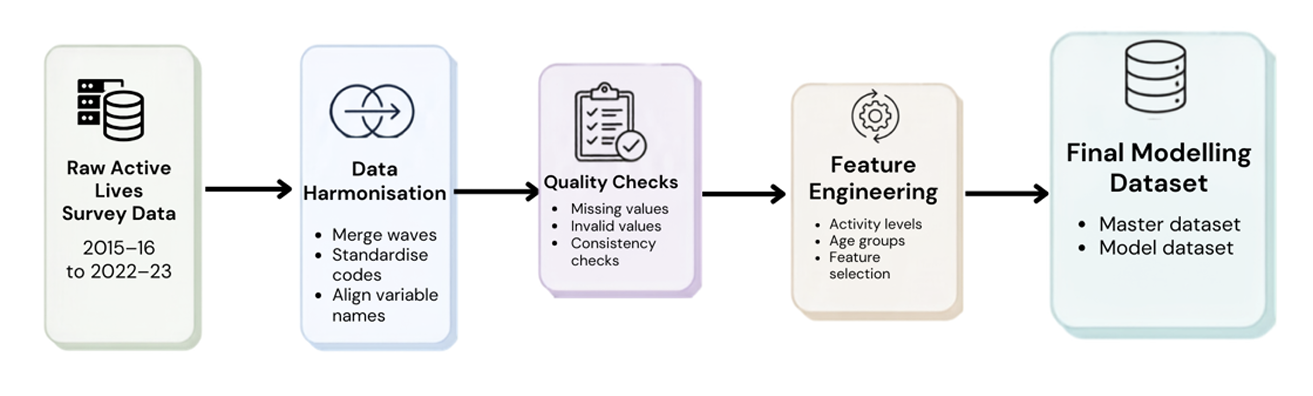
\includegraphics[width=0.85\textwidth]{figures/fig3_1_data_preprocessing_workflow.png}
\captionsetup{justification=centering}
\caption{Data preprocessing workflow showing dataset harmonisation, data quality checks, feature engineering, and creation of the final modelling datasets.}
\label{fig:preprocessing}
\end{figure}

\noindent
\textbf{Feature engineering.} After these checks, the cleaned 610-column master dataset was used to create smaller model-specific datasets. The main outcome, \texttt{Activity\_Level}, was used in an ordered three-category variable: 0:Inactive, 1:Fairly Active, and 2:Active. The demographic predictors were consolidated into consistent categories covering characteristics such as age, gender, ethnicity, disability, socio-economic group and education. Variables were selected according to their relevance to the four analytical pillars and the requirements of each modelling approach.

The resulting features provided a consistent basis for model development while retaining the demographic, geographical and behavioural information required for forecasting and scenario analysis.

\FloatBarrier
\section{Exploratory Data Analysis}

\noindent
Exploratory analysis was carried out to understand the main patterns in physical activity across London and to identify potential issues that could affect modelling. Activity levels varied considerably across boroughs, with clear differences also observed across demographic groups. In particular, age, socio-economic group and disability status showed noticeable associations with activity, while gender differences were comparatively smaller. These patterns provided an initial indication that demographic composition would be important when modelling participation.

Temporal analysis also showed changes in activity across the survey period, including a clear disruption during the COVID-19 period. This supported the use of time-based validation and forecasting approaches, rather than treating all survey waves as interchangeable observations.

\begin{figure}[!htb]
\centering
\includegraphics[width=0.75\textwidth]{figures/fig3_2_activity_levels_by_year.png}
\caption{Population-weighted distribution of activity levels across survey years}
\label{fig:activity-trends}
\end{figure}

Borough-level analysis further showed that differences in activity were not explained entirely by demographic composition. Some variation remained between boroughs after accounting for observed characteristics, supporting the inclusion of borough-level effects in the modelling framework.

\begin{figure}[!htb]
\centering
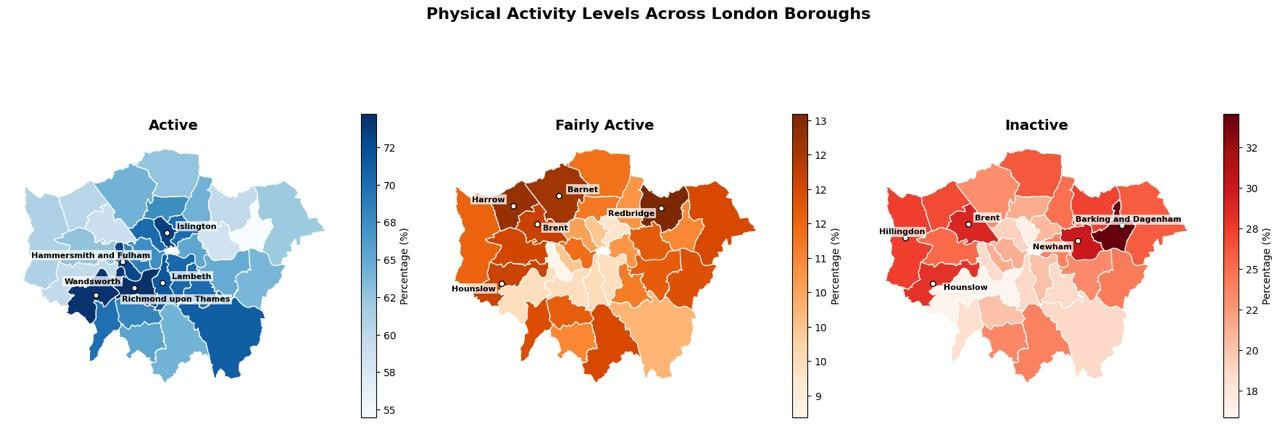
\includegraphics[width=\textwidth]{figures/fig3_3_borough_activity_variation.jpeg}
\caption{Geographical variation in population-weighted activity levels across London's boroughs.}
\label{fig:borough-variation}
\end{figure}

The EDA also identified differences in the availability and consistency of certain survey measures across waves. Variables such as indoor/outdoor activity, volunteering and free-time constraints were available for fewer years than the core activity measures. Consequently, these measures were used selectively in later analysis rather than being treated as consistent long-term forecasting variables.

Overall, the EDA established three important features of the data: strong demographic differences, meaningful temporal variation, and remaining borough-level variation. These findings informed the choice of modelling approaches and the subsequent forecasting framework.

\FloatBarrier
\section{Modelling Framework}

\noindent
Four complementary modelling approaches were developed to examine physical activity from statistical and machine-learning perspectives: CatBoost with SHAP, ordinal logistic regression benchmarked against LightGBM, K-Modes clustering with classification, and a Bayesian hierarchical ordinal model. All approaches used the same prepared survey data, but their outcome definitions and modelling objectives differed. CatBoost was used for individual-level prediction and interpretation, ordinal logistic regression and LightGBM were compared as alternative propensity models for the forecasting framework, the clustering approach explored respondent segments, and the Bayesian model represented the ordered Activity Level outcome and borough-level variation.

\FloatBarrier
\subsection{Prediction Targets and Notation}

\noindent
Let \(X_i\) represent the predictor variables for respondent \(i\), and let \(Y_i\) denote their physical activity outcome. For the binary prediction task, the outcome was defined as whether the respondent met the 150-minute physical activity guideline:

\[
Y_i =
\begin{cases}
1, & \text{if respondent meets the guideline} \\
0, & \text{otherwise}.
\end{cases}
\]

The corresponding predicted probability is denoted by

\[
p_i = P(Y_i = 1 \mid X_i).
\]

This probability represents the model's estimated likelihood that respondent \(i\) meets the guideline.

For the ordinal modelling task, physical activity was represented using the three-level \texttt{Activity\_Level} variable:

\[
Y_i \in \{0,1,2\},
\]

where 0 = Inactive, 1 = Fairly Active and 2 = Active. This preserves the natural ordering of the activity categories rather than treating them as unrelated classes.

\FloatBarrier
\subsection{Survey Weighting}

\noindent
The Active Lives Survey uses survey weights to account for the sampling design and improve the representativeness of estimates. Where supported by the modelling method, these weights were incorporated during model training. For an observation \(i\) with survey weight \(w_i\), a weighted loss can be expressed generally as

\[
\mathcal{L} = \sum_{i=1}^{n} w_i \,\ell(y_i,\widehat{y}_i),
\]

where \(\ell\) represents the loss for an individual observation. Consequently, observations with larger survey weights contribute more to the model's objective. This was particularly important when developing population-level predictions from the survey data.

\FloatBarrier
\subsection{Model Specifications}

\noindent
\textbf{Ordinal logistic regression} was used as the principal propensity model for
the forecasting framework and was benchmarked against LightGBM to assess
whether a more flexible non-linear model provided a meaningful improvement
in predictive performance. The model uses the three ordered Activity-Level
categories Inactive, Fairly Active and Active and estimates the cumulative
probability of being at or below each activity level. This provides a direct
and interpretable representation of the ordered outcome. The model was fitted
using the same predictor set and survey weights as the LightGBM benchmark.
Its main limitation is the proportional-odds assumption, which requires the
effect of each predictor to be consistent across the cumulative activity
thresholds.

LightGBM was used as the benchmark alternative to the ordinal logistic
propensity model. It is a gradient-boosting algorithm that builds a sequence
of decision trees, with each tree improving the errors made by the previous
trees. The prediction can be represented as,

\[
\widehat{y}_i = \sum_{k=1}^{K} f_k(X_i),
\]

where \(f_k\) represents an individual decision tree and \(K\) is the total number of trees. This approach is suitable for the survey data because it can capture non-linear relationships and interactions between demographic, temporal and activity-related predictors, and it served as a strong comparison against the ordinal logistic model used in the forecasting framework.

\textbf{CatBoost} was used as a second gradient-boosting approach for comparison. It is designed to handle categorical predictors effectively and can model non-linear relationships without requiring the same level of manual transformation as conventional regression models. SHAP values were additionally used with CatBoost to examine the contribution of individual predictors to model predictions.

\textbf{K-Modes Clustering and Classification} was used to group respondents according to similarities in their categorical demographic and activity characteristics. Unlike supervised prediction, clustering does not require a predefined outcome. The resulting clusters were then used as the target for a supervised classifier to assess how reliably cluster membership could be predicted from respondent characteristics. This provided a population-segmentation perspective rather than a direct forecasting model.

\textbf{Bayesian Hierarchical Ordinal Model} directly treated \texttt{Activity\_Level} as an ordered outcome and incorporated borough-level variation through a hierarchical structure. The linear predictor was defined as

\[
\eta_i = \beta^{T}X_i + u_{b[i]},
\]

where \(\beta\) represents the effects of the observed predictors and \(u_{b[i]}\) represents the random effect for the borough containing respondent \(i\). The cumulative probability of belonging to category \(k\) was modelled as

\[
P(Y_i \leq k) = \operatorname{logit}^{-1}(\theta_k-\eta_i),
\]

where \(\theta_k\) represents the ordered thresholds between activity categories. This allows the model to account for both individual characteristics and differences between boroughs while retaining the ordinal structure of the outcome.

\FloatBarrier
\subsection{Model Evaluation}

\noindent
Model performance was assessed using metrics appropriate to the prediction task. Accuracy measures the proportion of correctly classified observations, while Precision and Recall measure the reliability and completeness of positive predictions. Their harmonic mean is summarised by the F1-score:

\[
F1 = 2\frac{\mathrm{Precision}\times\mathrm{Recall}}
{\mathrm{Precision}+\mathrm{Recall}}.
\]

For probabilistic predictions, Log Loss measures how close the predicted probabilities are to the observed outcomes:

\[
\mathrm{LogLoss}
=
-\frac{1}{N}
\sum_{i=1}^{N}
\left[
y_i\log(p_i)
+
(1-y_i)\log(1-p_i)
\right].
\]

Lower Log Loss indicates better-calibrated probabilistic predictions. AUC measures the model's ability to distinguish between respondents who meet and do not meet the activity threshold across different classification thresholds, with a value of 0.5 representing random discrimination and higher values indicating better discrimination.

Where applicable, MAE and RMSE were also used for forecasting error:

\[
MAE =
\frac{1}{N}
\sum_{i=1}^{N}
\left|y_i-\widehat{y}_i\right|
\]

and

\[
RMSE =
\sqrt{
\frac{1}{N}
\sum_{i=1}^{N}
(y_i-\widehat{y}_i)^2
}.
\]

MAE gives the average absolute prediction error, while RMSE places greater emphasis on larger errors. These measures were used where the model produced continuous forecasts, while classification metrics were retained for models producing categorical or probabilistic outcomes.

\FloatBarrier
\section{Model Validation}

\noindent
Model validation was designed to assess how well the models generalise to observations that were not used during training. Since the data are collected across consecutive survey waves, a time-based validation strategy was used rather than a random train--test split. This ensures that information from later years is never used to predict an earlier year. For the forecasting framework, this validation was applied to the selected ordinal logistic propensity model.

\FloatBarrier
\subsection{Temporal Holdout}

\noindent
The final survey wave, 2022--23, was retained as an unseen test set. Candidate models were developed using the preceding survey waves and evaluated on this final wave. This provides a realistic assessment of how the modelling framework performs when applied to a future observation.

\FloatBarrier
\subsection{Rolling-Origin Backtesting}

\noindent
A rolling-origin approach was additionally used to test whether the selected forecasting framework produced consistent forecasts across different points in time. At each forecast origin \(\tau\), the ordinal logistic propensity model was trained only on the waves available up to that point and used within the forecasting framework to predict the following wave:

\[
\text{Train on waves }1,\ldots,\tau
\rightarrow
\text{Forecast wave }\tau+1
\]

This process was repeated for the available clean forecast origins (\(\tau=3,6,7\)). Origins that would forecast a pandemic-disrupted wave were excluded from the headline assessment, as these unusual conditions could distort the comparison.

\begin{table}[!htb]
\centering
\label{tab:rolling-origin-validation}
\begin{tabular}{llll}
\toprule
\textbf{Forecast origin} &
\textbf{Training data} &
\textbf{Forecast target} &
\textbf{Used in headline results} \\
\midrule
Wave 3                  & Waves 1--3                  & Wave 4        & yes \\
Wave 6                  & Waves 1--6                  & Wave 7        & yes \\
Wave 7                  & Waves 1--7                  & Wave 8        & yes \\
Pandemic-target origins & Available historical waves & Pandemic wave & no \\
\bottomrule
\end{tabular}
\caption{Rolling-origin validation design}
\end{table}

\FloatBarrier
\subsection{Forecasting Baselines}

\noindent
Simple forecasting baselines were included to determine whether the modelling framework provided improvement over straightforward alternatives. Two benchmarks were considered:

\begin{itemize}
\item Persistence: each borough is assumed to remain at its most recently observed activity rate.
\item Drift: each borough is assumed to continue following its previously observed trend.
\end{itemize}

Model performance was expressed relative to these benchmarks using a skill score:

\[
\mathrm{Skill}
=
1-
\frac{\mathrm{MAE}_{\mathrm{model}}}
{\mathrm{MAE}_{\mathrm{benchmark}}}
\]

A positive skill score indicates that the model has lower forecasting error than the benchmark.

\FloatBarrier
\section{Forecasting Framework}

\noindent
The forecasting framework combines the ordinal logistic propensity model with projected demographic composition and behavioural trends to estimate future physical activity levels. The framework separates expected changes due to population composition from changes associated with behavioural trends, allowing forecasts to be interpreted as a combination of demographic and behavioural effects.

\FloatBarrier
\subsection{Forecasting equation}

\noindent
For borough \(b\) at time \(t\), the predicted activity rate is defined as:

\[
\widehat{r}_{b,t}
=
\sum_{c} s_{b,c,t}p_{b,c}
+
\delta_t
\]

where \(s_{b,c,t}\) is the projected population share of demographic cell \(c\) in borough \(b\), \(p_{b,c}\) is the estimated probability of being active for that demographic cell, and \(\delta_t\) represents the overall behavioural trend.

This can be understood as who lives in the borough \(\times\) how likely that group is to be active + changes in behaviour over time. The propensity model does not directly model temporal trends or extrapolate activity into future survey years. Instead, time-dependent changes are introduced separately through the projected population composition and behavioural trend.

\FloatBarrier
\subsection{Population projection}

\noindent
Demographic composition was projected using the historical survey data for each borough. For each demographic cell, the historical population share was modelled using a linear trend on the logit scale. Borough-specific trends were then shrunk towards the corresponding London-wide trend:

\[
\widetilde{m}_{b,c}
=
\lambda m_{b,c}
+
(1-\lambda)m_c^{London},
\qquad
\lambda=0.5
\]

The projected shares were then transformed back to proportions and normalised so that the demographic shares within each borough sum to one. This shrinkage reduces the risk of unrealistic long-term projections caused by extrapolating from only eight observations.

The projection therefore focuses on demographic characteristics that can be projected reliably from the available population structure. The forecasting framework does not assume that every survey variable can be projected into the future.

\FloatBarrier
\subsection{Behavioural effect}

\noindent
The behaviour effect represents changes in activity that cannot be explained by changes in the demographic composition of the population. It is estimated from the difference between the observed London activity rate and the rate predicted from the observed demographic composition:

\[
\delta_t
=
r_t^{obs}
-
\sum_c s_{c,t}p_c
\]

A trend is then fitted to this residual using the non-pandemic waves. The COVID-affected waves are treated separately so that the unusual disruption does not determine the long-term behavioural trend. In the analysis, the estimated non-pandemic behavioural change was approximately +0.23 percentage points per year, while the estimated pandemic effect was approximately $-2.07$ percentage points.

\FloatBarrier
\subsection{Decomposing forecast changes}

\noindent
The framework allows the change in activity between two periods to be separated into two components:

\[
\Delta r_b
=
\underbrace{
\sum_c \Delta s_{b,c}p_{b,c}
}_{\text{composition effect}}
+
\underbrace{
\Delta\delta
}_{\text{behaviour effect}}
\]

The composition effect therefore measures the change resulting from the population becoming demographically different, while the behaviour effect measures the change in activity among people of the same demographic type.

This distinction is important for interpretation because the two effects imply different policy responses. For example, an increase in the proportion of older residents may reduce the overall activity rate through composition, whereas increased participation among existing demographic groups represents behavioural improvement.

\FloatBarrier
\subsection{Forecast scenarios and aggregation}

\noindent
Future forecasts are produced by applying the projected demographic shares and behavioural trend to each borough. Borough-level estimates are then aggregated to obtain London-wide forecasts using the corresponding population shares.

Because behavioural change is the least certain component over a ten-year horizon, forecasts are interpreted as scenarios rather than precise predictions. Where the available data are insufficient to support a reliable future projection, the analysis reports descriptive findings instead. For example, free-time constraints are available only in the 2022--23 wave, while volunteering and indoor/outdoor measures have limitations in their coverage; these are therefore not treated as equivalent to the main physical-activity forecast.


% -----------------------------------------------------------------------------
\chapter{Results and Critical Evaluation}
\label{chap:evaluation}

\FloatBarrier
\section{Experimental Results and Validation}

\noindent
The modelling framework was evaluated using both the final unseen survey wave and rolling-origin backtesting. The final 2022--23 wave was kept separate from model development and provided the main test of how well the models generalised to a previously unseen period. In addition, rolling-origin validation was used to assess whether the forecasting approach remained reasonably consistent when predicting different survey waves rather than relying on a single holdout period.

The results show that the supervised models were able to identify meaningful patterns in physical activity from demographic and borough-level characteristics. However, the models differed in their objectives and outcome definitions, so their results cannot be interpreted as a single ranking based on one metric. Ordinal logistic regression, LightGBM and the Bayesian model predict the three ordered activity levels, whereas CatBoost and the clustering-based approaches use binary or cluster-based outcomes. The comparison therefore considers predictive performance alongside the suitability of each approach for the project's forecasting objective.

A simple forecasting baseline was also used as a reference point. The purpose of the baseline was to establish whether the modelling approach provided useful predictive information beyond what could be achieved by simply carrying forward recent activity levels or continuing an existing trend. This provides a more meaningful assessment of forecasting performance than considering model accuracy alone.

For classification models, performance was assessed using measures including AUC, accuracy, F1-score and Log Loss where available. AUC indicates how well the model distinguishes between different outcome groups, while accuracy and F1-score describe classification performance. Log Loss provides an assessment of the quality of the predicted probabilities. Where continuous forecasting errors were available, MAE and RMSE were also considered, with RMSE giving greater weight to larger errors.

\FloatBarrier
\section{Model Results and Critical Evaluation}

\noindent
The modelling approaches produced different strengths and limitations because they used different target formulations and modelling assumptions. Therefore, models were compared using predictive performance alongside their suitability for the project's forecasting objective.

\begin{table}[!htb]
\centering
\small
\resizebox{\textwidth}{!}{%
\begin{tabular}{lllllll}
\toprule
\textbf{Model} & \textbf{Target} & \textbf{AUC} & \textbf{Logloss} & \textbf{Accuracy} & \textbf{Macro F1} & \textbf{Runtime} \\
\midrule
Ordinal logistic regression & 3-band ordinal & 0.704 & 0.797 & 67.1\%* & 0.392 & 45 min \\
LightGBM & 3-band ordinal & 0.707 & 0.794 & 67.4\%* & 0.387 & 15 min 50 sec \\
CatBoost & Binary & 0.708 & 0.588 & 68.9\% & --- & --- \\
Random Forest -- clustering & Binary & --- & --- & 54\% & 0.428 & 0 min 14 sec \\
Gradient Boosting -- clustering & Binary & --- & --- & 67.9\% & 0.363 & 2 min 16 sec \\
Bayesian Hierarchical Ordinal$^{\dagger}$ & 3-band ordinal & 0.68 & 0.82 & 65\% & 0.57 & $\sim$96 min \\
\bottomrule
\end{tabular}}
\caption{Model-specific performance metrics}
\label{tab:model-results}
\end{table}
\footnotesize
\item \textit{Notes:} $^{*}$ Weighted accuracy. 
$^{\dagger}$ Bayesian results are based on a preliminary run using 200 posterior draws, 200 tuning iterations, and 2 chains; therefore, its metrics and runtime are not directly comparable with the other models and are included for indicative comparison only.


\FloatBarrier
\subsection{Predictive performance}

\noindent
Table 4.1 summarises the available predictive performance measures. The two models most directly relevant to the forecasting framework were ordinal logistic regression and LightGBM, both evaluated using the three-band Activity Level outcome. Ordinal logistic regression achieved an AUC of 0.704 and weighted accuracy of 67.1\%, while LightGBM achieved an AUC of 0.707 and weighted accuracy of 67.4\%. The small difference in performance indicates that the two models provided broadly similar predictive results. LightGBM offered greater flexibility for capturing non-linear relationships and interactions, while ordinal logistic regression provided a simpler and more interpretable representation of the ordered activity outcome.

The clustering approaches produced mixed results. Random Forest clustering achieved 54.0\% accuracy and a Macro F1 of 0.428, while Gradient Boosting clustering achieved 67.9\% accuracy and a Macro F1 of 0.363. The Bayesian hierarchical ordinal model achieved an AUC of 0.680, accuracy of 65.0\%, and Macro F1 of 0.570. These results highlight that the approaches serve different modelling purposes and are therefore not directly interchangeable.

\FloatBarrier
\subsection{Forecasting performance}

\noindent
The selected ordinal logistic propensity model, combined with the demographic-projection framework, was additionally evaluated using rolling-origin backtesting to assess its ability to forecast future activity rates. Across the clean forecast origins, it achieved a mean MAE of 2.74 percentage points, compared with 3.44 percentage points for the naïve baseline. The model achieved mean skill scores of +0.20 against the naïve baseline and +0.31 against the drift benchmark, indicating improved forecasting performance over these simple alternatives.

The CatBoost forecasting implementation produced a final 2022--23 borough-level MAE of 3.28 percentage points and RMSE of 4.03 percentage points across 32 boroughs. However, these results should not be treated as a direct error comparison: the ordinal logistic forecasting value is averaged across rolling forecast origins, whereas the CatBoost values represent the final forecast period.

\FloatBarrier
\subsection{Selection of the Ordinal Logistic Model}

\noindent
The ordinal logistic model was selected as the propensity model for the forecasting framework because it provided a strong fit with the project’s forecasting objective. Most importantly, the framework requires the three ordered activity categories---Inactive, Fairly Active and Active---and the ordinal (cumulative-logit) formulation represents this ordered structure directly. Its predictive performance was very similar to that of LightGBM (AUC 0.704 compared with 0.707), so it was preferred because of its greater simplicity and interpretability, while still providing performance suitable for the forecasting framework.

LightGBM and CatBoost remained important comparison models: their similar AUC demonstrates that the predictive relationships are not dependent on a single algorithm, which strengthens confidence in the selected model rather than diminishing it.

The selection of the ordinal logistic model therefore reflects its overall suitability for the forecasting framework, while the close agreement with LightGBM and CatBoost confirms that the predictive relationships are robust across modelling approaches. This choice involves a trade-off: the ordinal logistic model assumes proportional odds across the activity thresholds, whereas LightGBM is more flexible in capturing non-linear relationships and interactions but is less directly interpretable.

\begin{table}[!htb]
\centering
\small
\begin{tabular}{
>{\raggedright\arraybackslash}p{0.24\textwidth}
>{\raggedright\arraybackslash}p{0.28\textwidth}
>{\raggedright\arraybackslash}p{0.25\textwidth}
>{\raggedright\arraybackslash}p{0.17\textwidth}
}
\toprule
\textbf{Model} & \textbf{Strength} & \textbf{Limitation} & \textbf{Role} \\
\midrule
Ordinal Logistic Model & Three-band ordered formulation; simple and interpretable & Assumes proportional odds across bands & Main forecasting model \\
LightGBM & Strong predictive performance and three-band formulation & Lower interpretability & Comparison model \\
CatBoost & Competitive binary prediction & Binary target & Comparison model \\
Random Forest clustering & Simple segmentation & Lower predictive performance & Exploratory \\
Gradient Boosting clustering & Captures non-linear patterns & Lower Macro F1 & Exploratory \\
Bayesian hierarchical ordinal & Explicit ordinal structure & Higher computational cost & Methodological comparison \\
\bottomrule
\end{tabular}
\caption{Model characteristics and analytical roles}
\label{tab:model-selection}
\end{table}

\FloatBarrier
\section{Physical Activity and Volunteering Trends Over the Next Ten Years}

\noindent
This section reports the forecast of all the four analytical pillars: overall participation forecasts, demographic-specific insights, indoor versus outdoor activity, and volunteering in sport.

\noindent
\textbf{A note on forecasting versus description:}

Forecasting was applied only where the data provided sufficient evidence for reliable projection: the question had to be measured consistently across survey years, have adequate sample coverage, and show sufficient predictive structure from demographic variables. Overall activity, activity types, club membership and key demographic groups met all three criteria and were therefore forecast, with borough-level projections and quantified uncertainty.

Where these conditions were not met, results are presented descriptively rather than as forecasts, so that no figure implies more confidence than the data can support. Free time was asked only in the final wave, so there is no trend to project and it can only be described as a current snapshot. Volunteering was measured inconsistently, as its question base changed twice during the series, and demographics explain only around 15\% of the variation between boroughs-too weak a signal to drive a projection, so it is reported at London and demographic level rather than forecast. Indoor and outdoor activity was asked of just $\sim$30\% of respondents, a rotating subsample that leaves the estimates with considerably greater uncertainty, so it is described with only one cautious London-level projection. Health was unavailable in the early survey years, leaving only five years of data, two of them affected by COVID and excluded as atypical; the remaining three clean years are not sufficient to establish a reliable trend, so despite being the strongest single correlate of activity, it too is reported descriptively.

This distinction ensures that forecasts are supported by the available evidence rather than presenting uncertain estimates as precise future outcomes

\FloatBarrier
\subsection{P1 - Overall Participation Forecasts}

\noindent
\paragraph{Physical activity across London as a whole}
\noindent

The model projects broad stability in London’s overall activity levels in the near term. By 2025--26, around 64.9\% of adults are projected to be Active, while 26.0\% are Inactive and 9.1\% are Fairly Active. Although the Active share changes little, the Fairly Active group has declined steadily over the observed period, suggesting a gradual shift away from the middle activity band.

\begin{figure}[!htb]
\centering
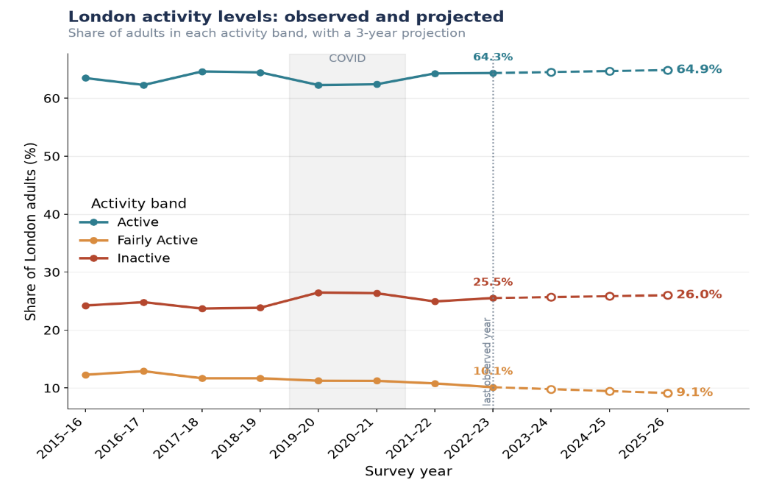
\includegraphics[width=0.85\textwidth]{figures/figP1_1_london_activity_bands.png}
\caption{London-wide activity bands, observed 2015--16 to 2022--23 and projected to 2025--26}
\label{fig:p1-1}
\end{figure}

\begin{table}[!htb]
\centering
\small
\begin{tabular}{lll}
\toprule
\textbf{Component} & \textbf{Effect by 2025--26} & \textbf{Interpretation} \\
\midrule
Composition & $-0.37$ points & London’s ageing population pulls activity down \\
Behaviour & +0.69 points & People of a given type are becoming more active \\
Net & +0.32 points & Apparent stability produced by two real trends cancelling \\
\bottomrule
\end{tabular}
\caption{Decomposition of the near-term London-wide forecast into composition and behaviour effects.}
\label{tab:p1-2}
\end{table}

This decomposition is the central analytical result behind the ‘stable’ headline. A conventional forecast would report the number as roughly flat and stop there. Decomposing it shows that the stability is a coincidence of two genuine trends cancelling, not a settled equilibrium. If the behavioural improvement stalls, the demographic headwind takes over. The stability is more fragile than the flat line suggests.

For the longer-term outlook, three scenarios are presented rather than a single point forecast. By 2031--32, the Active share ranges from approximately 61.0\% under a trend-reversal scenario to 65.4\% if recent gains continue, with a population-change-only scenario at around 63.1\%. This range highlights that the long-term direction of physical activity is sensitive to the assumptions made about future behaviour.

\begin{figure}[!htb]
\centering
\includegraphics[width=0.9\textwidth]{figures/figP1_2_ten_year_scenarios.png}
\caption{Ten-year scenario range for London-wide activity, 2022--2032}
\label{fig:p1-2}
\end{figure}

\newpage

\noindent
\paragraph{Likelihood of participating in specific activities}
\noindent

Ten-year scenario and three-year scenario ranges were produced for seven individual activities and three club-membership measures. Among them the top two activities are: Walking and Active Travel.

\begin{table}[!htb]
\centering
\small
\resizebox{\textwidth}{!}{%
\begin{tabular}{lrrrr}
\toprule
\textbf{Activity / Club Type} & \textbf{Today} & \textbf{If Gains Continue} & \textbf{Population Change Only} & \textbf{If Gains Reverse} \\
\midrule
Walking & 75.7\% & 71.4\% & 74.6\% & 71.5\% \\
Active travel & 60.2\% & 49.1\% & 58.6\% & 45.1\% \\
Fitness activities & 35.4\% & 31.8\% & 34.5\% & 29.5\% \\
Cycling & 19.7\% & 20.1\% & 18.9\% & 17.2\% \\
Team sports & 8.2\% & 6.5\% & 7.7\% & 4.9\% \\
Dance & 8.9\% & 5.2\% & 8.7\% & 7.0\% \\
Racket sports & 6.1\% & 5.1\% & 6.0\% & 4.0\% \\
Club membership (any sport)* & 16.3\% & 20.1\% & 15.6\% & 16.5\% \\
Fitness club / gym & 10.0\% & 9.4\% & 9.5\% & 9.5\% \\
Team-sport club & 4.7\% & 7.1\% & 4.3\% & 4.7\% \\
\bottomrule
\end{tabular}}
\caption{Ten-year scenario range by activity/club type (\% of London adults).}
\label{tab:p1-1}
\begin{tablenotes}[flushleft]
\footnotesize
\textit{Note:} * Club membership figures represent separate, potentially overlapping breakdowns rather than components of a single total. ``Fitness club/gym'' and ``team-sport club'' do not sum to ``club membership (any sport)'', since a person could belong to both, or to a club type not itemised here.
\end{tablenotes}

\end{table}



Continuing recent trends suggests a decline in most individual activities, except cycling, while all three club-membership measures show potential growth. However, this recovery is uneven: team-sport club membership shows the strongest increase (4.7\% $\rightarrow$ 7.1\%), whereas fitness/gym membership remains broadly flat or declines (10.0\% $\rightarrow$ 9.4\%). The wide scenario ranges for team sports and active travel reflect their strong disruption during COVID, so these long-term projections should be interpreted as directional rather than precise forecasts.

\noindent
\paragraph{Forecasts of activity levels for each London borough}
\noindent


Applying the ordinal logistic propensity model to each borough’s projected demographic composition produces a 2025 borough-level forecast ranging from 51.3\% in Barking and Dagenham to 75.4\% in Wandsworth.

The roughly 24-percentage-point gap between the most and least active boroughs is expected to persist throughout the projection period. The non-overlapping confidence intervals suggest that this difference is unlikely to be due to sampling variation alone. In addition, all 32 boroughs show a negative composition effect, ranging from close to zero to around $-0.9$ percentage points, indicating that projected demographic changes are expected to place some downward pressure on activity levels across London, although the size of this effect varies between boroughs.

\begin{figure}[!htb]
\centering
\begin{minipage}[t]{0.55\textwidth}
\centering
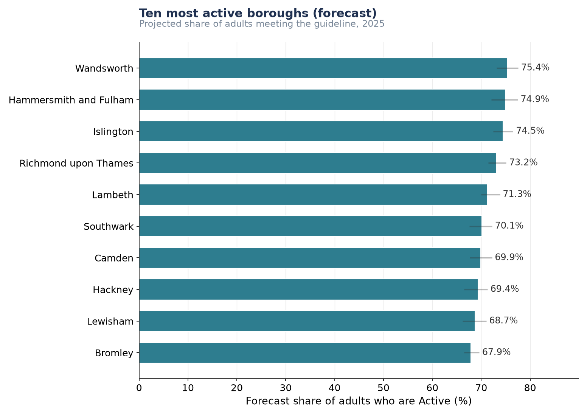
\includegraphics[width=\linewidth]
{figures/figP1_3a_most_active_boroughs.png}
\end{minipage}
\hfill
\begin{minipage}[t]{0.52\textwidth}
\centering
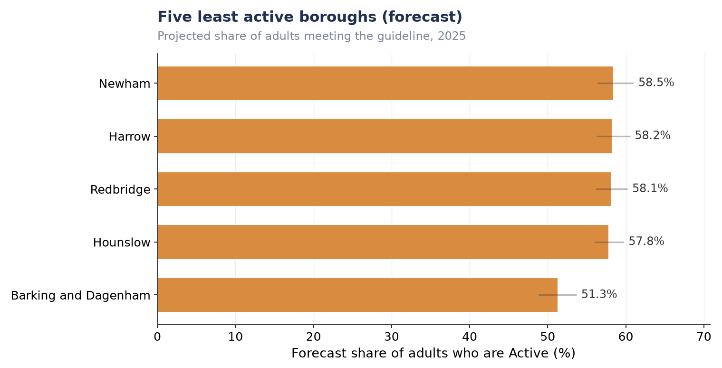
\includegraphics[width=\linewidth]{figures/figP1_3b_least_active_boroughs.png}
\end{minipage}
\caption{Ten most active boroughs \& five least active boroughs, projected share of adults meeting the guideline, 2025.}
\label{fig:p1-3}
\end{figure}


\newpage
\noindent
\paragraph{Key factors that may reduce free time and affect participation}
\noindent

Free-time constraint questions were asked once, in the 2022--23 wave only, of approximately a third of respondents. This section is therefore necessarily a cross-sectional snapshot rather than a ten-year forecast.

\begin{figure}[!htb]
\centering
\begin{minipage}[t]{0.51\textwidth}
\centering
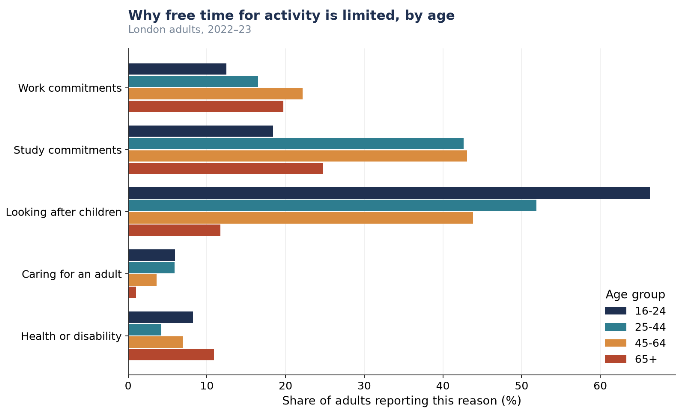
\includegraphics[width=\linewidth]{figures/figP1_4a_free_time_constraints.png}
\end{minipage}
\hfill
\begin{minipage}[t]{0.48\textwidth}
\centering
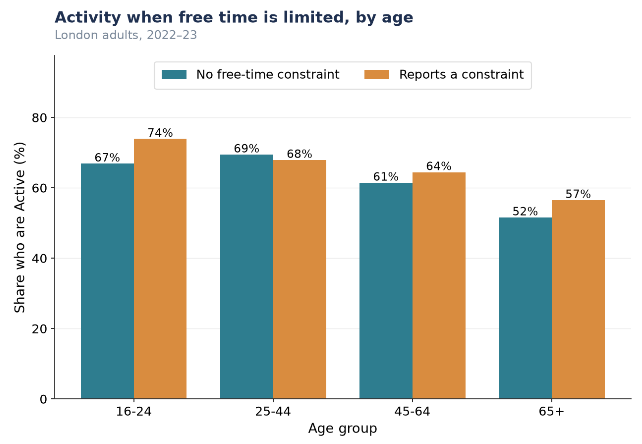
\includegraphics[width=\linewidth]{figures/figP1_4b_activity_by_constraint.png}
\end{minipage}
\caption{Reasons free time for activity is limited \& Activity rate by whether free time is constrained, (London adults, 2022--23).}
\label{fig:p1-4}
\end{figure}

The results show that work, study and childcare are the main reported constraints on free time, particularly among working-age adults, while caring responsibilities and health or disability are less frequently reported. However, reporting any free-time constraint was not associated with lower overall activity; constrained respondents were slightly more likely to be Active. This should be interpreted as a descriptive association rather than a causal relationship, as different constraints may have opposing effects. In particular, long working hours show a clearer negative association with physical activity, while activities such as childcare or active travel may themselves involve physical activity.

\FloatBarrier
\subsection{P2 - Demographic-Specific Insights}

\noindent
\paragraph{Forecasted participation levels by demographic group}
\noindent


\begin{figure}[!htb]
\centering
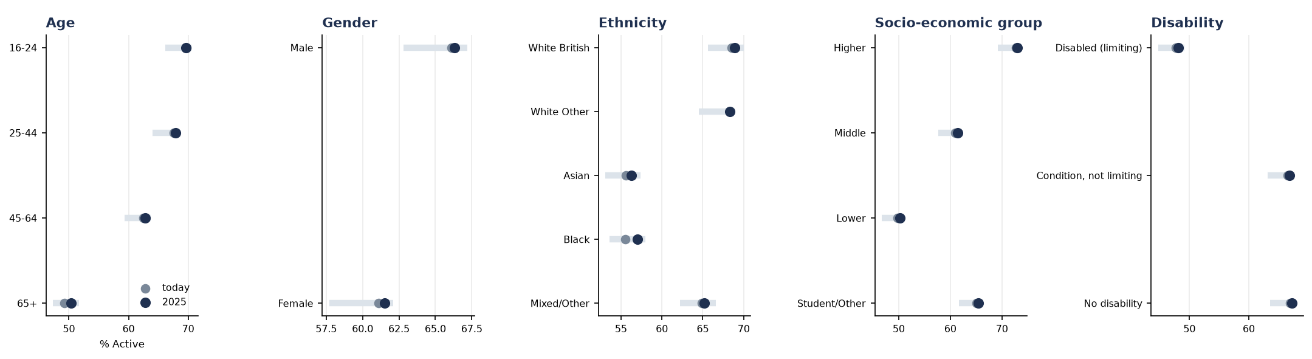
\includegraphics[width=\textwidth]{figures/figP2_1_demographic_forecast.png}
\caption{Activity forecast by demographic group; bar = 3-year forecast range, dot = today’s rate.}
\label{fig:p2-1}
\end{figure}

The forecast shows clear differences in physical activity across demographic groups, with socio-economic position showing the widest gap: around 73\% activity among the Higher group compared with 50\% in the Lower group (23 percentage points). This is followed by the age gap of around 20 points (70\% among 16--24 vs 50\% among 65+), the disability gap of 19 points, and the ethnicity gap of 13 points. Gender shows the smallest difference, at around 4 points (66\% male vs 62\% female). The 65+ group is particularly important, as it is both the least active group and shows little projected change (around +1 percentage point), meaning London's ageing population may create a demographic headwind to overall activity levels.

\noindent
\paragraph{Types of sport or physical activity each group is most likely to engage in}
\noindent


\begin{figure}[!htb]
\centering
\begin{minipage}[t]{0.38\textwidth}
\centering
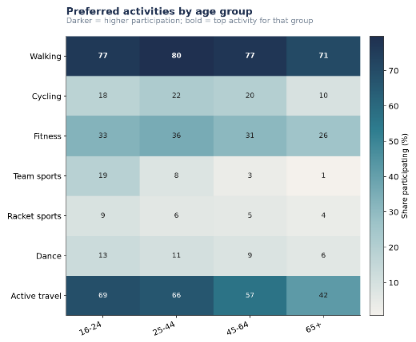
\includegraphics[width=\linewidth]{figures/figP2_2a_activity_by_age.png}
\end{minipage}
\hfill
\begin{minipage}[t]{0.38\textwidth}
\centering
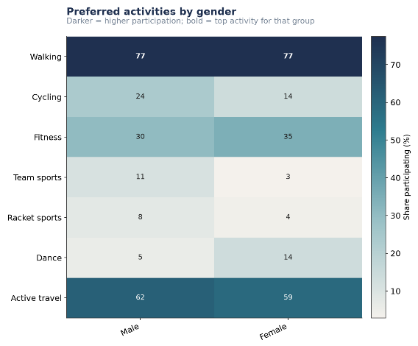
\includegraphics[width=\linewidth]{figures/figP2_2b_activity_by_gender_ethnicity.png}
\end{minipage}
\hfill
\begin{minipage}[t]{0.38\textwidth}
\centering
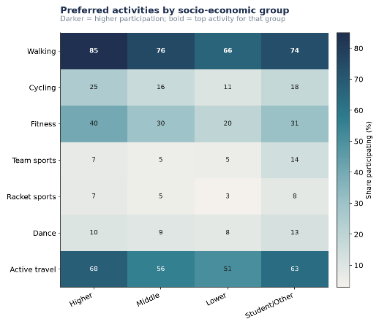
\includegraphics[width=\linewidth]{figures/figP2_2c_activity_by_socioeconomic_disability.png}
\end{minipage}
\caption{Which activities each group does most; bold marks the top activity for that group.}
\label{fig:p2-2}
\end{figure}

Walking is the most common activity across all demographic groups, although participation is lowest among adults with a limiting disability (64\%). The strongest age gradient occurs in team sports, falling sharply from 19\% among 16--24-year-olds to just 1\% among those aged 65+, while active travel, the second most common activity also declines from 69\% to 42\%. Gender differences vary by activity: men participate more in cycling, team and racket sports, while women lead in fitness and particularly dance (14\% vs 5\%), with walking equal at 77\%. Ethnic differences are also activity-specific, with Black respondents showing the highest participation in both dance (16\%) and team sports (10\%), while Asian respondents have the lowest fitness (26\%) and active travel (54\%) rates.

Socio-economic position shows particularly large differences in facility-dependent activities, with fitness at 40\% in the Higher group versus 20\% in the Lower group and cycling at 25\% versus 11\%. However, team sports are highest among the Student/Other group (14\%), while dance varies relatively little across socio-economic groups. Similarly, adults with a limiting disability have the lowest participation across all seven activities, with particularly large gaps in fitness, racket sports and active travel, but almost no gap in dance. Overall, dance stands out as the exception: unlike most other activities, it shows relatively small socio-economic and disability differences, suggesting that activities requiring greater access to facilities, equipment or organised provision are more strongly associated with demographic inequalities.

\noindent
\paragraph{Participation within each London borough}

\noindent

\textbf{Data note:} the ask was for participation in specific activities within each borough. However, the details for activity-type $\times$ borough was not available at reportable cell sizes. Thus, the provided plot is broken down by age-group participation within each borough. Borough-by-demographic cells are small: a single borough-by-age cell contains around six respondents in a given wave. All eight waves were therefore pooled and thin cells suppressed.

The 65+ group is the least active in all 32 boroughs, but the youngest group is not always the most active. In 11 boroughs, 25--44 matches or exceeds 16--24, most notably in Borough 012 (Hackney), where activity rises from 64\% (16--24) to 76\% (25--44). The age gap also varies considerably between boroughs, from 29 points in Borough 027 (Richmond upon Thames) (84\% vs 55\%) to just 11 points in Borough 014 (Haringey) (65\% vs 54\%). Borough 032 (Wandsworth) has the highest 65+ rate (59\%), while 002 (Barking and Dagenham) has the lowest (36\%), showing that borough-level differences can reinforce the effect of age.

\noindent
\paragraph{Likelihood of participation among people with health conditions}

Self-rated health is available from 2018--19 onwards (only 5 years data with 2 years of covid); the health-condition measures apply to people with a limiting disability. Results are descriptive, not forecasts.

\begin{figure}[!htb]
\centering
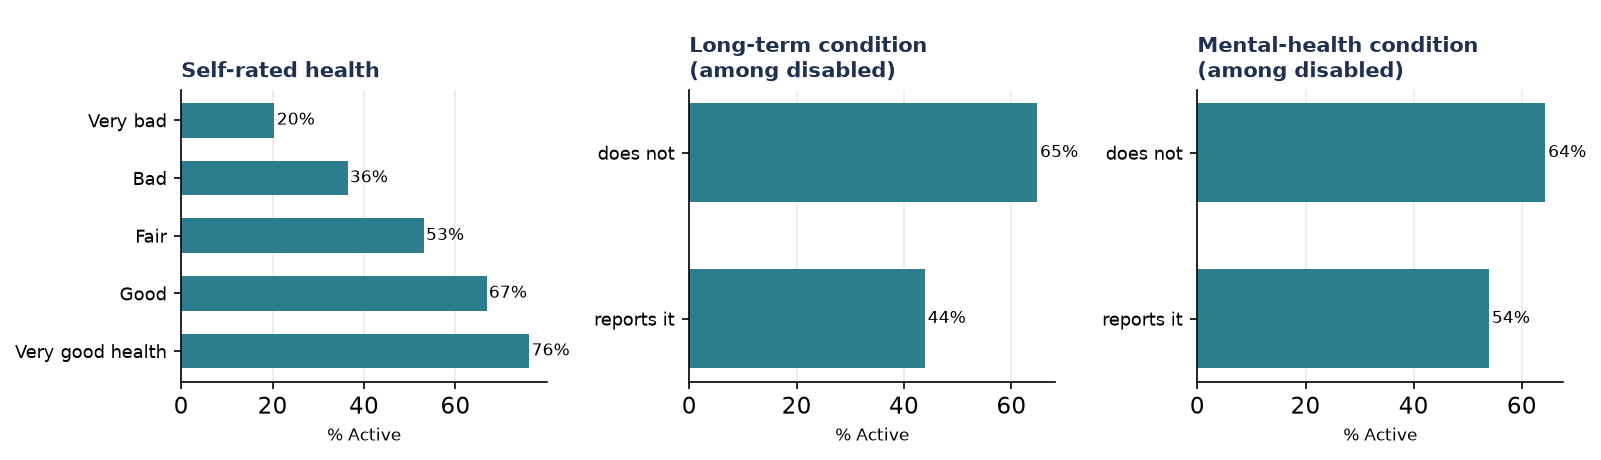
\includegraphics[width=1.0\textwidth]{figures/figP2_4_health_activity.png}
\caption{Activity by self-rated health, long-term condition and mental-health condition}
\label{fig:p2-4}
\end{figure}

Activity shows a strong and consistent health gradient, falling from 76\% among those reporting very good health to 20\% among those reporting very bad health. Among people with a limiting disability, those reporting a long-term condition are 21 percentage points less active than those without one (44\% vs 65\%), while the gap for mental-health conditions is smaller at 10 points (54\% vs 64\%). These results show a clear association between poorer health conditions and lower physical activity, although they do not establish causation.

\FloatBarrier
\subsection{P3 - Indoor vs Outdoor Activity}

\noindent
\paragraph{The expected balance of indoor versus outdoor physical activity}

The projection extends only to 2025 and is based on a $\sim$30\% subsample, so it should be treated as indicative rather than a full ten-year forecast.

\begin{figure}[!htb]
\centering
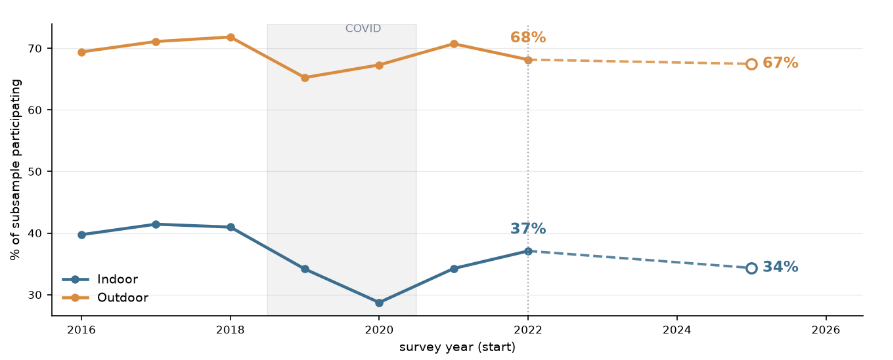
\includegraphics[width=0.85\textwidth]{figures/figP3_1_indoor_outdoor_trend.png}
\caption{Indoor vs outdoor activity over time, observed 2016--2022 and projected to 2025.}
\label{fig:p3-1}
\end{figure}

Outdoor activity remains substantially more common than indoor activity, at around 65--72\% compared with 29--42\% over the observed period. Both declined during COVID, but indoor participation fell more sharply, from 41\% in 2018 to 29\% in 2020, and had only partly recovered to 37\% by 2022. The indicative projection suggests indoor activity may fall further to 34\% by 2025, while outdoor activity remains broadly stable at 67\%, widening the gap between the two. However, this projection has a wide uncertainty range because it is based on the smaller subsample, so the figures should be interpreted directionally rather than as precise forecasts.

\noindent
\paragraph{Differences in indoor and outdoor activity preferences among people with varying activity levels}
\noindent
.

\begin{figure}[!htb]
\centering
\begin{minipage}[t]{0.32\textwidth}
\centering
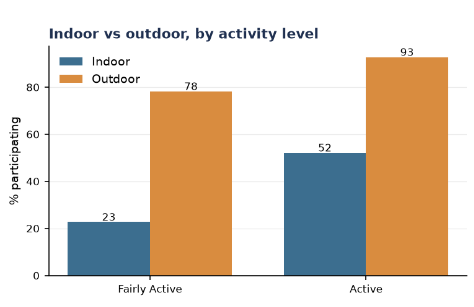
\includegraphics[width=\linewidth]{figures/figP3_2a_indoor_outdoor_preference.png}
\end{minipage}
\hfill
\begin{minipage}[t]{0.30\textwidth}
\centering
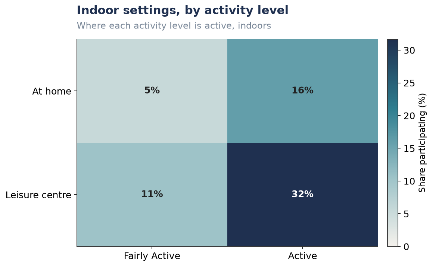
\includegraphics[width=\linewidth]{figures/figP3_2b_activity_locations.png}
\end{minipage}
\hfill
\begin{minipage}[t]{0.30\textwidth}
\centering
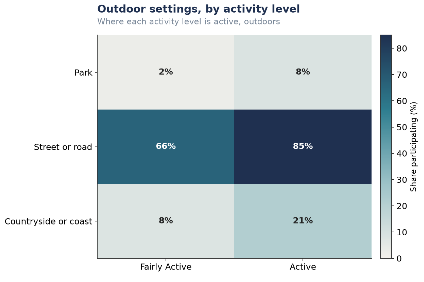
\includegraphics[width=\linewidth]{figures/figP3_2c_activity_level_locations.png}
\end{minipage}
\caption{Indoor/outdoor preference by activity level, and where each activity level is active.}
\label{fig:p3-2}
\end{figure}

Indoor activity differs much more by activity level than outdoor activity: Active respondents are more than twice as likely to participate indoors (52\% vs 23\%), while outdoor participation is already high (93\% vs 78\%). Street/road activity dominates outdoors (66\% vs 85\%) and changes least, whereas leisure-centre use shows the largest absolute increase (11\%$\rightarrow$32\%), followed by at-home activity (5\%$\rightarrow$16\%). Park and countryside/coast use also increase (2\%$\rightarrow$8\% and 8\%$\rightarrow$21\%). Overall, Fairly Active people mainly rely on accessible outdoor activity, while Active people are more likely to add indoor and a wider range of activity settings to their routine.

\noindent
\paragraph{Relationships between inner vs outer London locations, activity levels and socio-economic factors}
\noindent


\begin{figure}[!htb]
\centering
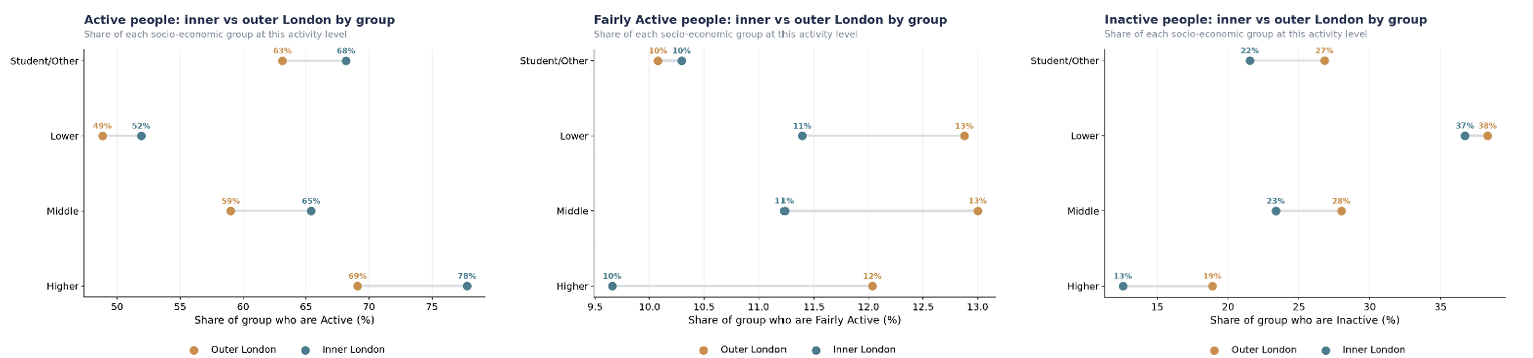
\includegraphics[width=\textwidth]{figures/figP3_3_inner_outer_socioeconomic.png}
\caption{Inner vs outer London $\times$ socio-economic group, indoor and outdoor activity.}
\label{fig:p3-3}
\end{figure}

Inner London generally has higher participation than Outer London across all socio-economic groups, but the gap is much smaller for the Lower group ($\sim$2--3 points) and wider for the Higher group, reaching around 10 points for outdoor activity. However, socio-economic differences are still stronger than location. Higher-income respondents in Outer London (40\% indoor; 73\% outdoor) remain more active than Lower-income respondents in Inner London (22\% indoor; 56\% outdoor). Overall, where people live matters, but socio-economic position appears to have the bigger influence.

\FloatBarrier
\subsection{P4 - Volunteering in Sport}

\noindent
Data Note: Volunteering cannot be reliably forecast because the survey question base changed across the years and demographics explain only around 15\% of borough-level variation. It is therefore reported descriptively rather than forecast at borough level.

\noindent
\paragraph{Current volunteering patterns across demographic groups}
\noindent

Volunteering is highest among younger adults, with 16--24-year-olds at 25\%, compared with 15\% among 65+. Men also volunteer more than women (21\% vs 15\%), while there is a clear socio-economic gradient (19\% Higher vs 12\% Lower). In contrast, volunteering varies much less by ethnicity and disability, ranging from 15--20\% across ethnic groups and 15--19\% by disability status. Overall, age, gender and socio-economic background show stronger differences than ethnicity or disability.

\begin{figure}[!htb]
\centering
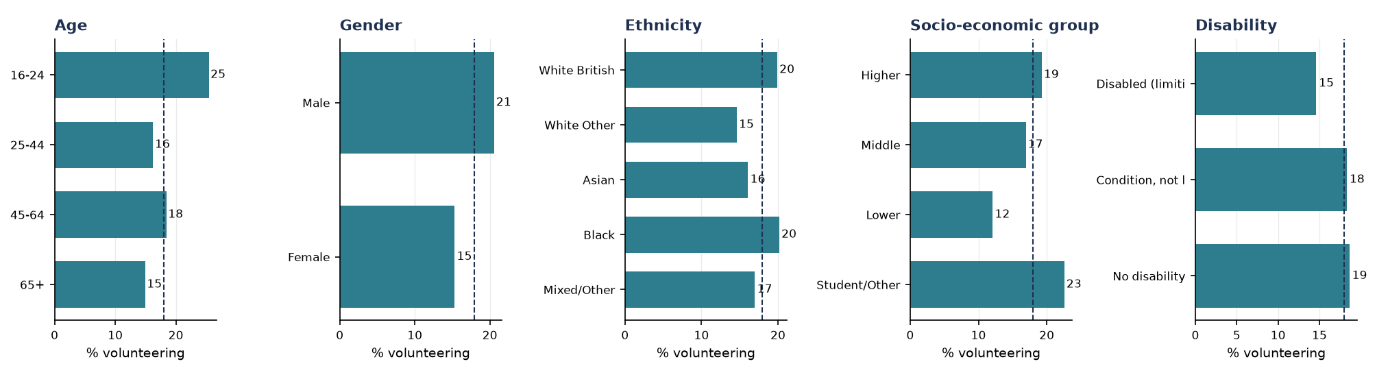
\includegraphics[width=0.9\textwidth]{figures/figP4_1_volunteering_background.png}
\caption{Volunteering in sport by background, pooled across waves. Described, not forecast.}
\label{fig:p4-1}
\end{figure}

\newpage

\noindent
\paragraph{Volunteer role patterns across demographic groups}
\noindent

\begin{figure}[!htb]
\centering
\begin{minipage}[t]{0.43\textwidth}
\centering
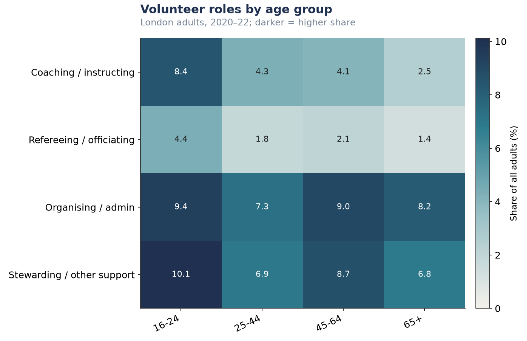
\includegraphics[width=\linewidth]{figures/figP4_2a_volunteer_roles.png}
\end{minipage}
\hfill
\begin{minipage}[t]{0.43\textwidth}
\centering
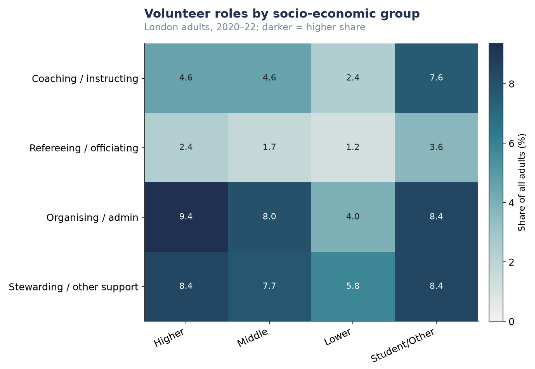
\includegraphics[width=\linewidth]{figures/figP4_2b_volunteer_roles_demographics.png}
\end{minipage}
\caption{Volunteer roles by demographic group, waves 2020--22}
\label{fig:p4-2}
\end{figure}

Organising/administration is the most consistent volunteer role across demographic groups, particularly among middle- and higher-income groups and most ethnicities. Younger adults stand out for more hands-on roles, with 16--24s highest in stewarding (10.1\%) and coaching (8.4\%). There is also a clear gender difference: men are more represented in coaching, officiating and stewarding, while women are more concentrated in organising and support. Lower socio-economic and some disability groups also show relatively higher reliance on stewarding/support roles.

\FloatBarrier
\section{Critical Discussion}

\noindent
The results provide a consistent picture of physical activity across London. Overall activity is relatively stable, but this stability reflects two opposing effects. An ageing population creates a demographic headwind, while activity levels within demographic groups have generally improved. The estimated $-0.37$ percentage-point composition effect is partly offset by a +0.69 percentage-point behavioural effect. This suggests that maintaining current activity levels may become more challenging as London's population changes.

The demographic results also show clear differences in participation between groups. Socio-economic group shows the widest overall gap, with age and disability also showing substantial differences. The 65+ group is particularly important because it is both the least active and the group showing the smallest improvement over time. These differences are also seen at borough level, where the age gradient remains present across all 32 boroughs. This suggests that demographic characteristics and where people live can work together to shape participation.

These findings have several practical implications for London Sport and local authorities. A single intervention is unlikely to address all of the differences observed. Walking and active travel provide an important low-barrier foundation, while activities such as fitness, cycling and structured sport show larger socio-economic and disability gaps. Improving access to facilities, clubs and suitable local infrastructure could therefore help address some of these differences. The relatively even pattern in volunteering also suggests that volunteering opportunities could provide another way of engaging people from a wider range of backgrounds.

The forecasts should, however, be treated as indicative estimates rather than precise predictions. The Active Lives Survey is repeated cross-sectional data, meaning that the analysis captures changes in the population rather than following the same individuals over time. The forecasting period is also based on a limited number of clean annual observations, with COVID-19 affecting several activity measures. Population projections introduce further uncertainty, while behavioural projections assume that historical patterns provide a reasonable indication of future change. The principal propensity model also assumes proportional odds across the three activity bands, which simplifies the modelling of the ordered outcome but may not fully capture differences in predictor effects between activity thresholds. Some outcomes, including volunteering and health-related measures, were therefore reported descriptively rather than forecast.

Overall, the findings suggest that future activity in London will be shaped by both changes in the population and the opportunities available to people. Demographic ageing is difficult to change directly, but the behavioural and place-related factors identified in this analysis provide areas where policy and investment can make a difference. The forecasts are therefore most useful for identifying which groups and areas may need greater attention and where interventions could have the greatest potential impact, rather than as exact predictions of London's future activity levels.



% -----------------------------------------------------------------------------

\chapter{Conclusion}
\label{chap:conclusion}

\section{Summary of Contributions}

The Active Lives Survey is built to describe what has already happened, and it does that well. It is not built to say what will happen next. A new sample of respondents is drawn each year, so there is no panel to follow, and eight annual waves give only 256 borough-year observations, three of which fall in the COVID-19 period. That is thin evidence for any conventional time-series method. This project worked around the problem rather than around the data, by estimating the relationship between individual characteristics and activity from the full sample of 135{,}497 respondents and introducing time separately, through projected population composition and an estimated behavioural trend.
The main contributions are as follows.

\paragraph{Harmonisation of eight structurally inconsistent survey waves.}
Local-authority identifiers were mapped to permanent ONS GSS codes so that the same 32 boroughs could be identified across every year. Sentinel codes were converted to missing values rather than treated as observations. Categories were reconciled where labels had changed but the underlying coding had not, as with the mid-level activity band renamed from Insufficiently Active to Fairly Active, and recoded where they genuinely differed, as with the additional NSSEC5 category folded into an existing one from 2019--20. Members of the team independently found borough codes that had been matched incorrectly between waves. That check was worth the time it took. A geographic mismatch produces no error message and no obviously wrong output, so it would have contaminated everything downstream
without ever announcing itself.

\paragraph{A comparison of the candidate modelling approaches under one
validation scheme.}
The ordinal logistic model, LightGBM, CatBoost with SHAP, K-Modes clustering with supervised classifiers, and a Bayesian hierarchical ordinal model were all developed on the same prepared data and tested on the same unseen 2022--23 wave. The predictive results were close: AUC of 0.704 for the ordinal logistic model, 0.707 for LightGBM and 0.708 for CatBoost. The agreement is itself a finding. It indicates that the demographic signal in the data is real but bounded, and that
it does not depend on the choice of algorithm.

\paragraph{Selection of the ordinal logistic model as the propensity component of the framework.}
It represents the three ordered activity bands directly, its coefficients can be read without additional tooling, and it behaves predictably when projected populations are passed through it. Its predictive performance was very similar to that of the gradient-boosting models, so the selection involved a small trade-off in predictive performance in favour of greater simplicity and interpretability.

\paragraph{A forecasting framework that separates composition from behaviour.}
Borough activity rates are built up from cell-level propensities weighted by projected demographic shares, with a behavioural term estimated from the
non-pandemic waves and added on top. Rolling-origin backtesting across the clean forecast origins gave a mean absolute error of 2.74 percentage points against 3.44 for the persistence baseline, with skill scores of $+0.20$ against the naive persistence benchmark and $+0.31$ against drift. The framework therefore does better than simply carrying the last observed rate forward, which is the comparison that matters for a method intended to be used.

\paragraph{The decomposition result itself.}
By 2025--26 the composition effect is $-0.37$ points and the behavioural effect $+0.69$ points, for a net of $+0.32$. London's overall activity rate looks flat, and a conventional forecast would report it as flat and stop. What the decomposition shows is that the flatness is a coincidence of two genuine trends pulling in opposite directions. If behavioural improvement stalls, the demographic pull takes over. This is the most useful result the project produced for a stakeholder, because it changes what stability means in practice.

\paragraph{Application across four analytical pillars with an explicit rule for when to forecast.}
Overall activity, activity types, club membership and the main demographic groups were forecast. Free-time constraints, volunteering, indoor and outdoor activity and health were reported descriptively, because each fails at least one of the three conditions the project set: consistent measurement across years, adequate sample coverage, and enough predictive structure from the demographic variables. Publishing a projection for volunteering would have been easy and would have looked no different on the page. It would also have implied a confidence the data cannot support.

\section{Evaluation Against Aims and Objectives}

All five objectives set out in Chapter~\ref{chap:introduction} were met, though two of them deserve some qualification.

Objective 1, harmonisation, is documented in Chapter ~\ref{chap:methodology} and produced the merged dataset of 135{,}497 respondents on which everything else rests.

Objective 2, developing and comparing candidate models and selecting one for the framework, was met, but the selection was a judgement rather than a result forced by the numbers. LightGBM had the higher AUC on the three-band target, by 0.003. The difference was small, so the decision came down to the other criteria: the ordinal formulation matches the outcome the framework needs, the coefficients are directly interpretable to the intended audience, and the model is stable when projected populations are pushed through it. A reader who weighted raw predictive accuracy more heavily could defend the opposite choice. It is worth being clear that this was a trade-off and not a ranking.

Objective 3, examining how far borough differences are associated with
demographic composition, was addressed through the exploratory analysis and the Bayesian hierarchical model. Borough-level variation did not disappear once observed demographic characteristics were accounted for, which justified treating geography as a separate component of the framework. What the analysis cannot do is say what that residual variation consists of. Calling it a place effect names it without explaining it.

Objective 4, the forecasting framework, is the project's central methodological contribution. It responds directly to the constraint that ruled out conventional time-series methods, and the backtesting in Chapter~\ref{chap:evaluation} shows it improves on both simple baselines rather than merely being more elaborate than them.

Objective 5, application and accessible presentation, was met across all four pillars, with the forecast-versus-describe distinction applied consistently.

The overall aim was to build an interpretable borough-level framework for
analysing and forecasting participation across London. That was achieved. The 2025 borough forecasts range from 51.3\% in Barking and Dagenham to 75.4\% in Wandsworth, a gap of roughly 24 percentage points that the projections expect to persist, and every one of the 32 boroughs carries a negative composition effect. Both results can be explained to a non-technical audience without reference to the model that produced them, which was the point.

\section{Limitations}

The repeated cross-sectional design is the binding constraint. The analysis
describes how the population changes, not how individuals change. When the
framework reports a behavioural improvement within a demographic group, it cannot distinguish between the same sort of people becoming more active and the composition of that group shifting in ways the demographic cells do not capture.

The behavioural trend rests on a small number of observations. Three of the eight waves were affected by the pandemic and were held out of the trend fit, leaving an estimate of roughly $+0.23$ percentage points per year drawn from very few clean years. A single unusual wave would move that number noticeably, and it carries directly into every forecast the framework produces.

The propensity model does not directly model temporal trends or extrapolate activity into future survey years. Instead, time-dependent changes are introduced separately through the projected population composition and behavioural trend. If the relationship between demographic characteristics and activity shifts, for instance if the 65+ group becomes substantially more active than earlier cohorts at the same age, the framework will absorb this into the behavioural residual rather than into the propensities themselves. It will take several further waves before such a change is visible.

The ordinal logistic propensity model also assumes proportional odds across the three activity bands. This means that the effect of each predictor is assumed to be consistent across the thresholds between Inactive, Fairly Active and Active. If predictor effects differ between these thresholds, the model may not fully capture the underlying relationships.

Population composition was projected by trending survey-based demographic shares on the logit scale, with borough trends shrunk halfway towards the London-wide trend. The shrinkage is a reasonable guard against extrapolating wildly from eight points, but the value of 0.5 was chosen for stability rather than calibrated against an external benchmark, and the projections are not official ONS or GLA population projections.

Borough differences remain unexplained. Without data on facility density, green space, transport provision and local deprivation at a matching resolution, the analysis can show that boroughs differ after demographics are accounted for but cannot say why.

An AUC of around 0.70 means demographic characteristics predict individual behaviour only moderately well. That is adequate for the aggregate shares the framework produces, since errors at the individual level largely cancel across a borough population. It is not adequate for any claim about a particular person.

Several outcomes could not be forecast. Volunteering was measured on a changing question base and demographics account for only around 15\% of borough-level variation in it. Indoor and outdoor activity was asked of roughly 30\% of respondents through a rotating subsample. Free-time constraints appear in one wave only. Health, despite being the strongest single correlate of activity found anywhere in the analysis, is available for five years, two of which were excluded as atypical. Borough-by-demographic cells are also thin, at around six respondents per cell per wave, which is why all eight waves had to be pooled for that breakdown.

\section{Future Work}

The most direct extension is to bring in external borough-level data. Facility density, green space, cycling infrastructure and deprivation measures could be added as borough covariates to test whether the residual geographic variation shrinks once they are included. That would turn the place effect from a label into something with content, and would tell London Sport whether the differences between boroughs are mainly about provision or about something else.

Replacing the survey-based population trending with official sub-national population projections would remove one source of uncertainty and would make the composition effect easier to defend to a statistically literate stakeholder.

The Bayesian hierarchical model was the natural home for forecast uncertainty but was held back by runtime, which reached around 96 minutes for a single fit. A more efficient implementation, whether through a reparameterised model or variational inference, could move it from a corroborating role to the primary source of interval estimates, so that borough forecasts carry credible intervals derived from the model rather than approximated separately.

A further methodological extension would be to assess alternatives to the proportional-odds assumption used by the ordinal logistic propensity model. Models that allow predictor effects to vary across the thresholds between Inactive, Fairly Active and Active could be compared with the current formulation to determine whether the additional flexibility provides a meaningful improvement in predictive performance.

As further waves are released, the measures currently reported descriptively should be revisited. Volunteering and the indoor and outdoor split need a longer run of consistent questions before they can be forecast, and the same applies to the health measures, which would be the most valuable addition of the three given how strongly health relates to activity.

Finally, the framework currently answers the question of what happens if present trends continue. Stakeholders will also want to know what happens if a particular intervention is made. Answering that would mean linking policy levers to cell-level propensities, which requires evidence about intervention effects that the Active Lives Survey does not contain. It would be a different project, but the framework built here provides a reasonable place to attach it.

For London Sport, the practical message is not the headline forecast. It is that the headline is stable for two reasons that could easily stop cancelling each other out, that the gap between the most and least active boroughs is wide and shows no sign of closing on its own, and that the activities where boroughs differ most are the ones that depend on facilities and organised provision. Those are the parts of the picture that can actually be acted on.




% =============================================================================

% Finally, after the main matter, the back matter is specified.  This is
% typically populated with just the bibliography.  LaTeX deals with these
% in one of two ways, namely
%
% - inline, which roughly means the author specifies entries using the 
%   \bibitem macro and typesets them manually, or
% - using BiBTeX, which means entries are contained in a separate file
%   (which is essentially a database) then imported; this is the 
%   approach used below, with the databased being dissertation.bib.
%
% Either way, the each entry has a key (or identifier) which can be used
% in the main matter to cite it, e.g., \cite{X}, \cite[Chapter 2}{Y}.

\backmatter

\bibliography{sample_bibtex}

% -----------------------------------------------------------------------------

% The dissertation concludes with a set of (optional) appendices; these are 
% the same as chapters in a sense, but once signalled as being appendices via
% the associated macro, LaTeX manages them appropriately.

\appendix

\chapter{Supplementary Methods and Validation}
\label{appx:supplementary-methods}

\noindent
\emph{Concepts, equations and results supporting the methodology and validation chapters}

\noindent
This appendix documents the components of the analysis that are referenced in, or underpin, the main methodology and results but are not set out there in full. Each section states the concept, the relevant equation where applicable, and the result obtained on the real data. Together they complete the white-box account of how the forecasts were produced and validated.

\section{External validation of the activity bands}

\noindent
The three-band activity outcome (Inactive 0--29, Fairly Active 30--149, Active 150+ weekly moderate-equivalent minutes) was derived directly from the minutes measure rather than taken from a survey-supplied grouping. Deriving it independently permits a direct external check against Sport England's own published classification of the same underlying measure.

\noindent
\textbf{Result:} the derived classification reproduced Sport England's published grouping with 100\% agreement in every one of the eight survey waves. Because this single check exercises the file merge, the recoding and the outcome definition simultaneously against a reference the analysis did not control, it is the foundational validation on which all downstream results rest.

\section{Non-disclosure as an informative category}

\noindent
The optional demographic questions were declined by some respondents. Rather than dropping or imputing these cases, non-disclosure was retained as an explicit category, because disclosure behaviour is itself strongly predictive of activity.

\begin{table}[!htb]
\centering
\begin{tabular}{lcc}
\toprule
\textbf{Disclosure behaviour} & \textbf{Share of sample} & \textbf{\% meeting the guideline} \\
\midrule
Disclosed all optional items & 88.1\% & 65.7\% \\
Withheld one item & 11.0\% & 48.0\% \\
Withheld two or more items & 1.0\% & 28.2\% \\
\bottomrule
\end{tabular}
\end{table}

\noindent
\textbf{This is a 37-percentage-point gradient --- wider than the effect of age, ethnicity or socio-economic group.} Whatever non-disclosure captures (survey engagement, language, institutional trust), it predicts inactivity more strongly than any demographic variable in the data. Imputing or dropping these respondents would overstate activity in every subgroup, so retaining ``Not disclosed'' as a level is both more honest and more accurate.

\section{Data-quality audit: four corrected defects}

\noindent
Systematic cross-wave screening --- comparing each variable's coverage and prevalence wave by wave and flagging abrupt shifts --- uncovered four defects, each of which would have produced confident but wrong results, and none of which was visible by casual inspection.

\begin{table}[!htb]
\centering
\small
\begin{tabularx}{\textwidth}{@{}lXXX@{}}
\toprule
\textbf{Defect} & \textbf{What was wrong} & \textbf{Artefact if missed} & \textbf{Correction} \\
\midrule
Club-membership base & Asked of sport players most years, but of everyone in the final year & Membership appears to collapse 36\% $\rightarrow$ 16\% & Rebased to all adults; incomparable early waves excluded \\
Volunteer-role base & Asked of all until 2019--20, then of volunteers only & Coaching appears to rise fivefold, 5\% $\rightarrow$ 26\% & Rebased to all adults; roles restricted to consistent waves \\
Health variable & Absent in the first three waves & Becomes a disguised indicator of which wave a respondent came from & Excluded from all models; used only for description \\
Implausible activity & 146 respondents report more weekly minutes than a week contains & Distorts group averages & Winsorised at a defensible ceiling \\
\bottomrule
\end{tabularx}
\end{table}

\noindent
\emph{These checks are a permanent part of the pipeline: a future year's data is screened the same way automatically, and any new structural break is flagged rather than silently absorbed.}

\section{Composition versus place: the decomposition of borough variation}

\noindent
Before forecasting, it must be settled whether differences between boroughs are driven by who lives there (composition) or by the place itself, since only the first responds to population change. Let \(r^b\) be borough \(b\)'s observed activity rate and \(\hat{r}^b\) its rate predicted from demographics alone. The share of between-borough variation explained by composition is the coefficient of determination across boroughs:

\[
R^2_{\mathrm{comp}}
=
1-
\frac{\sum_b (r^b-\hat{r}^b)^2}
{\sum_b (r^b-\bar{r})^2}
\]

Three models were compared on the held-out wave, and the demographic-only model was additionally evaluated leave-one-borough-out (each borough predicted by a model trained without it):

\begin{table}[!htb]
\centering
\begin{tabularx}{\textwidth}{@{}Xc@{}}
\toprule
\textbf{Model} & \textbf{Share of between-borough spread reproduced} \\
\midrule
Demographics only & 48\% \\
Borough identity only & 86\% \\
Demographics and borough together & 88\% \\
Demographics only, on boroughs never seen in training & 47\% \\
\bottomrule
\end{tabularx}
\end{table}

\noindent
\textbf{Result:} roughly half of the difference between boroughs is compositional and half is not. The final row is decisive --- the demographic model predicts a borough it has never encountered (47\%) almost as well as one it trained on (48\%), which is precisely the property that licenses using demographic projection to forecast populations that do not yet exist. Place effects do not offset composition but amplify it: the demographic model ranks boroughs almost perfectly (correlation 0.90) yet understates the size of the gaps, so disadvantaged boroughs are penalised twice --- once by demography and once by environment.

\section{The provision gradient}

\noindent
Repeating the composition-versus-place decomposition across fifteen behaviours produced the project's clearest strategic finding: the more a behaviour depends on facilities and provision, the less of its geography demographics explain.

\begin{table}[!htb]
\centering
\begin{tabular}{lclc}
\toprule
\textbf{Follows the people (composition-led)} & & \textbf{Follows the place (provision-led)} & \\
\midrule
Walking & 50\% & Volunteering & 15\% \\
Overall activity & 48\% & Park use & 18\% \\
Fitness activities & 45\% & Team-sport club & 25\% \\
Outdoor activity & 45\% & Cycling & 29\% \\
Indoor activity & 44\% & Leisure-centre use & 31\% \\
\bottomrule
\end{tabular}
\end{table}

\noindent
\textbf{The ordering is not arbitrary.} Walking requires only a pavement and tracks the population closely; cycling requires lanes and storage; park and racket sports require facilities; volunteering requires organisations to volunteer for. The strategic implication is direct: the behaviours least predictable from demographics are precisely those most open to influence through investment. Cycling, the behaviour with the widest borough gap in the dataset, is roughly 71\% attributable to place rather than population.

\section{Benchmarks and the skill score}

\noindent
A model's quality is meaningful only against a baseline. Two families of benchmark were used. For the classifier, the floor is a prevalence predictor that assigns the base rate to everyone (AUC 0.5 by construction); single-feature models give a stronger floor.

\begin{table}[!htb]
\centering
\begin{tabular}{lcl}
\toprule
\textbf{Benchmark} & \textbf{AUC} & \textbf{Interpretation} \\
\midrule
Prevalence (base rate for everyone) & 0.500 & The absolute floor \\
Age band alone & 0.572 & One predictor \\
Ethnicity alone & 0.568 & One predictor \\
Socio-economic group alone & 0.619 & Strongest single feature \\
Ordinal logistic propensity model & 0.704 & Clears any single feature by 0.085 \\
\bottomrule
\end{tabular}
\end{table}

For the forecast, the benchmarks are computed per borough: persistence (each borough held at its last value) and drift (each borough continuing its own trend). Model quality is then reported as a skill score --- the fractional reduction in error relative to a benchmark:

\[
\mathrm{Skill}
=
1-
\frac{\mathrm{MAE}_{\mathrm{model}}}
{\mathrm{MAE}_{\mathrm{benchmark}}}
\]

Skill \(>0\) means the method beats the benchmark; 0 means no better than trivial; \(<0\) means worse. Reporting skill rather than raw error makes ``the model is good'' an explicit, quantified comparison. The forecasting framework achieved skill of +0.20 against persistence and +0.31 against drift.

\section{Interval calibration}

\noindent
A point forecast is only half of a responsible forecast; the stated uncertainty must also be truthful. A 90\% interval should contain the actual value about 90\% of the time. Coverage is defined as the share of back-test cases whose actual value fell inside the predicted band:

\[
\mathrm{Coverage}
=
\frac{1}{N}
\sum_i
\mathbb{1}
\left[
lo_i \leq y_i^{actual} \leq hi_i
\right]
\]

\noindent
\textbf{Measured on the back-test, the original intervals covered the actual value only 53\% of the time --- substantially over-confident.} The cause was that the bootstrap captured only sampling uncertainty (which respondents were surveyed) and omitted process uncertainty (the genuine year-to-year variation of the world). The published bands were therefore missing an entire source of uncertainty, not merely too small.

The correction is principled, not cosmetic. The process standard deviation was measured empirically from the back-test's own one-step forecast errors (3.44 percentage points) and added to the sampling standard deviation in quadrature:

\[
\sigma_{\mathrm{total}}
=
\sqrt{\sigma_{\mathrm{samp}}^2+\sigma_{\mathrm{proc}}^2}
\qquad
90\% \text{ interval}
=
\hat{r}
\pm
1.645\,\sigma_{\mathrm{total}}
\]

\begin{table}[!htb]
\centering
\begin{tabular}{lc}
\toprule
\textbf{Interval basis} & \textbf{Measured 90\% coverage} \\
\midrule
Sampling only (original) & 53\% --- over-confident \\
Sampling + measured process variance (calibrated) & 94\% \\
\bottomrule
\end{tabular}
\end{table}

\noindent
\textbf{Note on honesty:} the widening was fixed by the measured process variance, not tuned to hit a target, and the resulting coverage (94\%, marginally conservative) was reported as it fell out. A result of exactly 90\% would in fact be more suspicious. The central forecasts are unchanged by calibration --- only the band widths.

\section{Decomposition of the uncertainty range}

\noindent
A complete uncertainty range reflects three separate sources: the survey happening to sample different people, the model's own coefficients being imperfect, and the genuine year-to-year variation of the process. The bootstrap refits the model on each resample, so it already captures the second source; its size was confirmed by isolating it.

\begin{table}[!htb]
\centering
\begin{tabularx}{\textwidth}{@{}XcX@{}}
\toprule
\textbf{Source} & \textbf{Contribution to the 90\% half-width (pp)} & \textbf{Role} \\
\midrule
Year-to-year process variation & 5.66 & Dominant --- the piece calibration adds \\
Survey sampling of people & 0.44 & Small \\
Model coefficient variability & 0.35 & Smallest --- but genuinely present \\
\bottomrule
\end{tabularx}
\end{table}

The model's own coefficient uncertainty is therefore not missing from the range; it is captured by the bootstrap and is the smallest of the three contributors. The dominant source is year-to-year process variation --- precisely what the calibration in Section G was built to include.

\section{Sensitivity to the shrinkage weight (\texorpdfstring{\(\lambda\)}{lambda})}

\noindent
The population projection blends each borough's own trend with the London-wide trend, in a balance set by a shrinkage weight \(\lambda\), fixed at a conservative midpoint of 0.5:

\[
\widetilde{m}_{b,c}
=
\lambda \cdot m_{b,c}
+
(1-\lambda)\cdot m_c^{London},
\qquad
\lambda=0.5
\]

To confirm this choice does not drive the result, the entire forecast was re-run across the full range of \(\lambda\), from 0 (each borough's own trend only) to 1 (the London trend only), both for the London headline and for every borough separately.

\noindent
\textbf{Result:} the choice of \(\lambda\) is immaterial. Across the whole range the London forecast moves by just 0.04 percentage points, and even the single most \(\lambda\)-sensitive borough, Waltham Forest, moves only 1.3 points; every other borough moves less. \(\lambda=0.5\) is therefore a safe, conservative default rather than an influential free parameter.

\section{Corroboration: forecasting for the right reason}

\noindent
A forecast can beat a benchmark by accident. The corroboration check tests whether it beats it for the reason claimed. Because the method forecasts a borough by projecting its demographic composition, it should forecast best on boroughs whose activity is demographically explained, and worst on boroughs driven by place effects it does not model. Writing \(|e^b|\) for a borough's composition residual (its place strength, Section D) and \(\mathrm{MAE}^b\) for its mean back-test error, the mechanism predicts a positive rank correlation:

\[
\rho
=
\mathrm{Spearman}
\left(
|e^b|,
\mathrm{MAE}^b
\right)
>
0
\]

\noindent
\textbf{Result:} the rank correlation is +0.74 (Pearson +0.65) --- a strong positive relationship. The boroughs the framework forecasts worst are precisely those where place dominates (for example Wandsworth and Camden), and the ones it forecasts best are those where demographics explain activity (for example Harrow and Merton). The forecast therefore succeeds through the demographic mechanism it claims, not by coincidence. With 32 boroughs and a small number of origins this is reported as strong corroborating evidence rather than proof.

\section{Validation summary}

\noindent
The three headline validation results, established on real data, are:

\begin{table}[!htb]
\centering
\begin{tabular}{lcl}
\toprule
\textbf{Validation result} & \textbf{Value} & \textbf{What it establishes} \\
\midrule
Forecast skill vs naïve & +0.20 & The forecast is accurate \\
Calibrated interval coverage & 94\% & The uncertainty is honest \\
Corroboration correlation & +0.74 & It is accurate for the right reason \\
\bottomrule
\end{tabular}
\end{table}

\noindent
\textbf{Taken together these establish that the forecast is accurate, that its stated uncertainty is truthful, and that its accuracy arises from the demographic mechanism the framework claims.} The remaining limitations --- principally the three clean back-test origins available from an eight-wave, two-pandemic-year series --- are constraints of the data rather than the method: the analysis is more rigorous than the data can fully reward, and the framework strengthens automatically as further survey years arrive.


% =============================================================================

\end{document}